%%%% Small single column format
\documentclass[anonymous=false, %
               format=acmsmall, %
               review=true, %
               screen=true, %
               nonacm=true]{acmart}

\usepackage{booktabs}       % professional-quality tables
\usepackage{amsfonts}       % blackboard math symbols
\usepackage{nicefrac}       % compact symbols for 1/2, etc.
\usepackage{microtype}      % microtypography
\usepackage{graphicx}
\usepackage{multirow}
\usepackage{amsmath}
\usepackage{amssymb}
\usepackage{subcaption}
\usepackage{paralist}
\usepackage{tabularx}
\usepackage{placeins}

% Import customized style files
\usepackage{algorithm}
\usepackage{algorithmicx}
\usepackage[noend]{algpseudocode}
\usepackage{setspace}
\usepackage{enumitem}
% operators

\newcommand{\argmax}{\operatornamewithlimits{argmax}}
\newcommand{\argmin}{\operatornamewithlimits{argmin}}

% vectors
\let\avec\vec
%\renewcommand{\vec}[1]{\ensuremath{\boldsymbol{#1}}}
\renewcommand{\v}[1]{\ensuremath{\boldsymbol{#1}}}

\newcommand{\src}{\lstinline[mathescape, keepspaces]}
\newcommand{\msrc}[1]{\mbox{\src!#1!}}

\newcommand{\tens}[1]{%
  \mathbin{\mathop{\otimes}\limits_{#1}}%
}

% symbol shorthands (lowercase)
%\newcommand{\x}{\ensuremath{\v{x}}}
%\newcommand{\y}{\ensuremath{\v{y}}}
%\newcommand{\z}{\ensuremath{\v{z}}}
%\newcommand{\h}{\v{\eta}}
%\newcommand{\e}{\v{\epsilon}}
%\renewcommand{\u}{\v{u}}
\newcommand{\pd}{\ensuremath{\partial}}
\newcommand{\x}{\ensuremath{x}}
\newcommand{\y}{\ensuremath{y}}
\newcommand{\z}{\ensuremath{z}}
\newcommand{\h}{\ensuremath{\eta}}
\newcommand{\e}{\ensuremath{\epsilon}}
\renewcommand{\u}{\ensuremath{u}}
\newcommand{\q}{\theta}
\newcommand{\f}{\phi}
\renewcommand{\l}{\lambda}
\renewcommand{\t}{\tau}

% symbol shorthands (uppercase)
\renewcommand{\L}{\ensuremath{\mathcal{L}}}
\newcommand{\KL}[2]{\ensuremath{\mathrm{KL}\left({#1} \:\middle\vert\middle\vert\: {#2}\right)}}
\newcommand{\E}{\ensuremath{\mathbb{E}}}
\newcommand{\N}{\ensuremath{\mathcal{N}}}
% \newcommand{\C}{\ensuremath{\mathtt{Concrete}}}

%\let\lmid\mid
%\renewcommand{\mid}{\!\lmid\!}

\newcommand{\eval}{\ensuremath{$\reflectbox{$\,\leadsto\,$}$}}
%\newcommand{\eval}{\sim}
\newcommand{\hide}[1]{}

\makeatletter
\DeclareRobustCommand{\cev}[1]{%
  \mathpalette\do@cev{#1}%
}
\newcommand{\do@cev}[2]{%
  \fix@cev{#1}{+}%
  \reflectbox{$\m@th#1\vec{\reflectbox{$\fix@cev{#1}{-}\m@th#1#2\fix@cev{#1}{+}$}}$}%
  \fix@cev{#1}{-}%
}
\newcommand{\fix@cev}[2]{%
  \ifx#1\displaystyle
    \mkern#23mu
  \else
    \ifx#1\textstyle
      \mkern#23mu
    \else
      \ifx#1\scriptstyle
        \mkern#22mu
      \else
        \mkern#22mu
      \fi
    \fi
  \fi
}

\renewcommand{\algorithmicrequire}{\textbf{Input:}}
\renewcommand{\algorithmicensure}{\textbf{Output:}}

\algnewcommand\algorithmicassert{\texttt{assert}}
\algnewcommand\Assert[1]{\State{} \algorithmicassert(#1)}

\algnewcommand\algorithmicswitch{\textbf{switch}}
\algnewcommand\algorithmiccase{\textbf{case}}
\algnewcommand\algorithmicdefault{\textbf{default}}
\algdef{SE}[SWITCH]{Switch}{EndSwitch}[1]{\algorithmicswitch\ #1\ \algorithmicdo}{\algorithmicend\ \algorithmicswitch}
\algdef{SE}[CASE]{Case}{EndCase}[1]{\algorithmiccase\ #1}{\algorithmicend\ \algorithmiccase}
\algdef{SE}[DEFAULT]{Default}{EndDefault}[1]{\algorithmicdefault\ #1}{\algorithmicend\ \algorithmicdefault}
\algtext*{EndSwitch}
\algtext*{EndCase}
\algtext*{EndDefault}

\algnewcommand\algorithmicmatch{\textbf{match}}
\algdef{SE}[MATCH]{Match}{EndMatch}[1]{\algorithmicmatch\ #1}{\algorithmicend\ \algorithmicmatch}
\algtext*{EndMatch}

\algnewcommand\algorithmictry{\textbf{try}}
\algnewcommand\algorithmiccatch{\textbf{catch}}
\algblockdefx[Try]{Try}{EndTry}{\algorithmictry}{\algorithmicend\ \algorithmictry}
\algtext*{EndTry}
\algcblockdefx[Catch]{Try}{Catch}{EndTry}[1]{\algorithmiccatch\ #1}{\algorithmicend\ \algorithmictry}%
\algtext*{EndTry}
\MakeRobust{\Call}

\algdef{SE}[QUERY]{Query}{EndQuery}%
   [2]{\textbf{query}\ \textproc{#1}\ifthenelse{\equal{#2}{}}{}{(#2)}}%
   {\algorithmicend\ \algorithmicquery}%
\algtext*{EndQuery}

\def\@algocf@capt@ruled{under}


\definecolor[named]{Blue}{cmyk}{1,0.1,0,0.1}
\definecolor[named]{Yellow}{cmyk}{0,0.16,1,0}
\definecolor[named]{Orange}{cmyk}{0,0.42,1,0.01}
\definecolor[named]{Red}{cmyk}{0,0.90,0.86,0}
\definecolor[named]{LightBlue}{cmyk}{0.49,0.01,0,0}
\definecolor[named]{Green}{cmyk}{0.20,0,1,0.19}
\definecolor[named]{Purple}{cmyk}{0.55,1,0,0.15}
\definecolor[named]{DarkBlue}{cmyk}{1,0.58,0,0.21}

\hypersetup{%
  colorlinks,
  linkcolor=Red,
  citecolor=DarkBlue,
  urlcolor=DarkBlue
}

\usepackage[acronym,smallcaps,nowarn,section,nogroupskip,nonumberlist]{glossaries}
\glsdisablehyper{}
\newacronym{SCFM}{scfm}{stochastic control-flow model}
\newacronym{WS}{ws}{wake-sleep}
\newacronym{BWS}{bws}{basic wake-sleep}
\newacronym{RWS}{rws}{reweighted wake-sleep}
\newacronym{ELBO}{elbo}{evidence lower bound}
\newacronym{VAE}{vae}{variational autoencoder}
\newacronym{IWAE}{iwae}{importance weighted autoencoder}
\newacronym{KL}{kl}{Kullback-Leibler}
\newacronym{SGD}{sgd}{stochastic gradient descent}
\newacronym{VIMCO}{vimco}{variational inference for Monte Carlo objectives}
\newacronym{WW}{ww}{wake-wake}
\newacronym{WWS}{wws}{wake-wake-sleep}
\newacronym{AIR}{air}{Attend, Infer, Repeat}
\newacronym{ESS}{ess}{effective sample size}
\newacronym{REINFORCE}{reinforce}{Reinforce gradient estimator}
\newacronym{IS}{is}{importance sampling}
\newacronym{GMM}{gmm}{Gaussian mixture model}
\newacronym{MNIST}{mnist}{hand-written digit dataset}
\newacronym{RELAX}{relax}{RELAX gradient estimator}
\newacronym{REBAR}{rebar}{REBAR gradient estimator}
\newacronym{PMF}{pmf}{probability mass function}
\newacronym{MLP}{mlp}{multilayer perceptron}
\newacronym{RNN}{rnn}{recurrent neural network}
\newacronym{PCFG}{pcfg}{probabilistic context free grammar}
\newacronym{ADAM}{adam}{ADAM}
\glsunset{ADAM}

\usepackage{amsthm}
\newtheorem{proposition}{Proposition}
\theoremstyle{definition}
\newtheorem{definition}{Definition}

\usepackage{xcolor}
\newcommand{\given}{\lvert}
\newcommand{\pw}{\overset{\text{p.w.}}{\sim}
}


%%%%%%%probprog style%%%%%%%%
% \usepackage[ruled]{algorithm2e} 
%\usepackage{parskip}
\urlstyle{tt}
\citestyle{acmauthoryear}

\begin{document}

\title{Amortized Population Gibbs Samplers with Neural Sufficient Statistics}
%  \titlenote{This is a titlenote}
%  \subtitle{This is a subtitle}
%  \subtitlenote{Subtitle note}

\author{Hao Wu}
%\orcid{1234-5678-9012-3456}
\affiliation{%
  \institution{Northeastern University}
  \department{Khoury College of Computer Science}
  %\streetaddress{43 Vassar St}
  \city{Boston}
  \state{MA}
  %\postcode{02115}
%   \country{USA}
}
\email{haowu@ccs.neu.edu}

\author{Heiko Zimmermann}
%\orcid{1234-5678-9012-3456}
\affiliation{%
  \institution{Northeastern University}
  \department{Khoury College of Computer Science}
  %\streetaddress{625 Mt Auburn St #3}
  \city{Boston}
  \state{MA}
  %\postcode{02115}
%   \country{USA}
}
\email{hzimmermann@ccs.neu.edu}

\author{Eli Sennesh}
%\orcid{1234-5678-9012-3456}
\affiliation{%
  \institution{Northeastern University}
  \department{Khoury College of Computer Science}
  %\streetaddress{15 Network Dr}
  \city{Boston}
  \state{MA}
  %\postcode{02115}
%   \country{USA}
}
\email{esennesh@ccs.neu.edu}

\author{Tuan Anh Le}
%\orcid{1234-5678-9012-3456}
\affiliation{%
  \institution{Massachusetts Institute of Technology}
  %\streetaddress{15 Network Dr}
  \city{Cambridge}
  \state{MA}
  %\postcode{02115}
%   \country{USA}
}
\email{tuananh@mit.edu}

\author{Jan-Willem van de Meent}
%\orcid{1234-5678-9012-3456}
\affiliation{%
  \institution{Northeastern University}
  \department{Khoury College of Computer Sciences}
  %\streetaddress{360 Huntington Ave}
  \city{Boston}
  \state{MA}
  %\postcode{02115}
%   \country{USA}
}
\email{j.vandemeent@northeastern.edu}
%\renewcommand\shortauthors{Mage, M. et al}

\begin{abstract}
We develop amortized population Gibbs (APG) samplers, a new class of autoencoding variational methods for deep probabilistic models. APG samplers construct high-dimensional proposals by iterating over updates to lower-dimensional blocks of variables. Each conditional update is a neural proposal, which we train by minimizing the inclusive KL divergence relative to the conditional posterior. To appropriately account for the size of the input data, we develop a new parameterization in terms of neural sufficient statistics, resulting in quasi-conjugate variational approximations. Experiments demonstrate that learned proposals converge to the known analytical conditional posterior in conjugate models, and that APG samplers can learn inference networks for highly-structured deep generative models when the conditional posteriors are intractable. Here APG samplers offer a path toward scaling up stochastic variational methods to models in which standard autoencoding architectures fail to produce accurate samples.
\end{abstract}

\maketitle

\section{Introduction}
%\vspace{-0.5em}

\label{introduction}

Deep probabilistic programming libraries such as Edward \cite{tran2016edward}, Pyro \cite{bingham2018pyro}, and Probabilistic Torch \cite{siddharth2017learning}  extend deep learning frameworks with functionality for deep probabilistic models. One commonly used class of models are 
% Both models are parameterized using neural networks, which are trained using stochastic gradient descent by optimize a lower or upper bound on the log marginal likelihood. 
% Training an inference network to perform amortized inference can be equivalently understood as a form of variational inference or adaptive importance sampling.
variational autoencoders (VAEs) \cite{kingma2013auto-encoding, rezende2014stochastic}, where the generative model (decoder) combines an unstructured prior (e.g.~a spherical Gaussian) with a likelihood that is parameterized by an expressive neural network, and the inference network (encoder) maps input data (e.g.~an image or sentence) onto an embedding vector, also known as the latent code.

Deep probabilistic programming aims to enable more general designs that incorporate structured priors for tasks such as multiple object detection \cite{eslami2016attend}, language modeling \cite{esmaeili2019structured}, or object tracking \cite{kosiorek2018sequential}. In these domains, a prior can incorporate useful inductive biases, which in turn can help guide a model to uncover patterns in the data in an unsupervised manner, and aid generalization in complex domains where the training data may not contain exemplars for all possible combinations of latent features.

However, training structured models also poses challenges that are not encountered in unstructured problems. To optimize a lower or an upper bound, we need to approximate the gradient of an expectation with a Monte Carlo estimate (see \cite{mohamed2019monte} for a recent review).
% Standard VAEs rely on reparameterized estimators that can often approximate the gradient with a single sample. 
Unfortunately, the gradient estimators can have a high variance in models where latent variables are high-dimensional and/or strongly correlated. Owing to these limitations, models that are trained using standard VAE objectives often consider relatively small-scale problems, such as tracking $\le 2$ objects over the course of 10 frames \cite{kosiorek2018sequential}.

In this paper, we develop methods for amortized inference that are designed to scale to structured models with 100s of latent variables. We are particularly interested in the frequently arising cases of models that are characterized by a combinations of \emph{local variables}, such as the time-dependent position of an object, and \emph{global variables}, such as the shape of the object. Our approach is similar in spirit to work by Johnson et al. \cite{johnson2016composing}, who perform inference using variational EM algorithms \cite{beal2003variational,bishop2006pattern,wainwright2008graphical} for conjugate-exponential models with a neural likelihood. 

Rather than requiring exact EM updates, we here propose a more general approach by defining an importance sampling method that employs conditional proposals to iterate between updates to blocks of variables. To train these conditional proposals, we define a variational method that minimizes the inclusive KL divergence between the proposal update and the exact conditional posterior. The difficulty lies in the gradient estimation, since the conditional posterior is in general intractable. To address this, we develop a sequential Monte Carlo sampler \cite{delmoral2006sequential} that combines approximate Gibbs updates with resampling steps in order to construct high quality proposals, which serve both to compute gradient estimates at train time and to perform inference at test time. We refer to the resulting class of methods as \emph{amortized Gibbs} samplers, since the proposals approximate Gibbs updates. 

Another challenge is the parameterization of these conditional proposals, which need to appropriately account for the amount of data on which we are conditioning. To address this difficulty, we propose a class of networks that we refer to as \emph{neural sufficient statistics}, which define parameterizations of proposals in a manner that is additive in the local variables, much like the sufficient statistics in conjugate-exponential families.

Our experiments show that learned proposals converge to the true conditional posteriors in Gaussian mixture models, where the Gibbs updates can be computed in closed form. Moreover we establish that amortized Gibbs methods serve can a basis for scalable inference in structured deep generative models, including mixtures with neural likelihoods and unsupervised tracking models. Both of these tasks are representative of the current state-of-the art in unsupervised approaches for learning structured deep generative models.
\section{Amortized Population Gibbs Samplers}
\label{sec:amortized-gibbs}
We are interested in the task of jointly training a generative model $p_\q(x, z)$ by maximizing its marginal likelihood $p_\q(x)$ and learning an inference model $q_\f(z \mid x)$ that approximates the posterior $p_\q(z \mid x)$. 
% Like most amortized inference approaches, we assume that we can sample from a (possibly implicit) distribution $\hat{p}(\x)$ that either takes the form of an empirical distribution over training data or a data simulator.
As a means of generating high-quality samplesin an incremental manner, we develop methods that are inspired by EM and classical Gibbs sampling, which perform iterative updates to blocks of variables. We here assume that the latent variables in the generative model decompose into blocks $\z = \{\z_1, \ldots, \z_B\}$ and train proposals $\log q_\f(z_b \mid x, z_{-b})$ that update the variables in a each block $z_{b}$ conditioned on the variables in the remaining blocks $\z_{-b} = z \setminus \{z_b\}$.

Starting with an initial sample from an encoder $q_\f(\z^{1} \mid \x)$, we will generate a sequence of samples $\{z^1, \ldots, z^K\}$ by performing conditional updates to each block $z_b$, which we refer to as a \emph{sweep}
\begin{align}
    \label{eq:approx-gibbs-kernel}
    q_\f \big( \z^k \mid \x, \z^{k-1} \big)
    &=
    \prod_{b=1}^B
    q_\f(\z^k_b \mid \x, \z^{k}_{\prec b}, \z^{k-1}_{\succ b})
    ,
\end{align}
where $\z_{\prec b} = \{z_i \mid i < b\}$ and $\z_{\succ b} = \{z_i \mid i > b\}$. Repeatedly applying sweep updates then yields a proposal
$
    q_\f(z^1, \ldots, z^K \mid x) 
    =
    q_\f(z^1 \mid x)
    \prod_{k=2}^K
    q_\f(z^k \mid \x, z^{k-1}).
$
% \begin{equation*}
%     q_\f(z^1, \ldots, z^K \mid x) 
%     =
%     q_\f(z^1 \mid x)
%     \prod_{k=2}^K
%     q_\f(z^k \mid \x, z^{k-1}).
% \end{equation*}
We want to train proposals that improve the quality of each sample $z^k$ relative to that of the preceding sample $z^{k-1}$. To accomplishing this, we learn a sweep update that leaves the target density \emph{invariant}
\begin{equation}
    \label{eq:kernel-invariance}
    p_\q(\z^k \,|\, \x) = \int \: p_\q(\z^{k-1} \,|\, \x) \: q_\f(\z^k \,|\,\x, \z^{k-1}) d z^{k-1}.
\end{equation}
When this condition is met, the proposal $q_\f(z^1, \ldots z^K \,|\, x)$ is a Markov Chain whose stationary distribution is the posterior. 
This means a sweep update learned at training time can be applied at test time to iteratively improve sample quality, without requiring a pre-specified number of updates $K$. In addition, when we require that each single block update $q_\f(z'_b \mid x, z_{-b})$ also leaves the target density invariant,
\begin{align}
    \label{eq:gibbs-invariance}
    p_\q(z'_b, z_{-b} \mid x)
    = 
    \int 
    p_\q(z_b, z_{-b} \mid x) \:
    q_\f(z'_b, \mid x, z_{-b}) 
    dz_{b}
    = 
    p_\q(z_{-b} \mid x) \:
    q_\f(z'_b \mid x, z_{-b})
    ,
\end{align}
Then we see that a block update must equal the exact conditional posterior, $q_\f(z'_b \mid x, z_{-b}) = p_\q(z'_b \mid x, z_{-b})$.
In other words, when the condition in Equation~\ref{eq:gibbs-invariance} is met, the proposal $q_\f(z^1, \ldots z^K \,|\, x)$ is a Gibbs sampler.


\subsection{Variational Objective} 
To learn each of the block proposals $q_\f(z_b \mid x, z_{-b})$ we minimize the inclusive KL divergence $\mathcal{K}_b(\f)$
\begin{align}
    \E_{\hat{p}(x)p_\q(z_{-b} | x)}
    \left[
    \text{KL}\left(
        p_\q(z_{b} \mid x, z_{-b})
        ||
        q_\f(z_{b} \mid x, z_{-b})
    \right)
    \right]. \label{eq:variational_objective}
\end{align}
Unfortunately, this objective is intractable, since we cannot evaluate the density of the true marginal $p_\q(z_{-b} \mid x)$, nor that of the conditional $p_\q(z_{b} \mid z_{-b}, x)$. 
% As we will discuss in Section~\ref{sec:experiments}, this has implications for the evaluation of learned proposals, since we cannot compute a lower or upper bound on the log marginal likelihood as in other variational methods. However, it nonetheless possible to approximate the gradient of the objective
However, we can nonetheless estimate this gradient using any Monte Carlo method that generates samples $z \sim p_\q(z \mid x)$ from the posterior. In the next section, we will use learned proposals to define an importance sampler, which we then use to compute an self-normalized estimator of the gradient from weighted samples $\{(w^l, z^l)\}_{l=1}^L$, 
\begin{align}
    \label{eq:grad-self-normalized}
    -\nabla_\f \mathcal{K}_b(\f)
    =
    \E_{
    \hat{p}(x) \:
    p_\q(z_{b}, z_{-b} | x)
    }
    \left[
    \nabla_\f
    \log q_\f(z_{b} \,|\, x, z_{-b})
    \right]
    \simeq
    \sum_{l=1}^L
    \frac{w^l}{\sum_{l'} w^{l'}}
    \nabla_\f
    \log q_\f(z^l_{b} \,|\, x, z^l_{-b})
    .
\end{align}
In problems where we would like to learn a deep generative model $p_\q(\x, \z)$, we can apply a similar self-normalized gradient estimator of the form
\begin{align}
    \label{eq:grad-theta}
    \nabla_\q \log p_\q(\x) 
    =
    \mathbb{E}_{p_\q(\z | \x)} 
    \left[
    \nabla_\q \log p_\q(\x, \z)
    \right]
    \simeq
    \sum_{l=1}^L
    \frac{w^l}{\sum_{l'} w^{l'}}
    \nabla_\q
    \log p_\q(x, z^l)
    .
\end{align}
This identity holds due to the property $\E_{p_\q(z|x)}[\nabla_\q \log p_\q(z|x)]=0$ (see Appendix \ref{appendix:grad-theta} for details). 

% The estimator in Equation~\ref{eq:grad-self-normalized} is similar to the self-normalized estimator in reweighted wake-sleep methods \cite{bornschein2014reweighted}, which also minimizes an inclusive KL divergence. This estimator has a number of advantages over the estimator that is commonly used to train standard VAEs, which minimize an exclusive KL divergence \cite{le2019revisiting}. Standard VAE objectives rely on reparameterization to compute gradient estimates. For discrete variables, reparameterization is not possible. This means that we need to compute likelihood-ratio estimators (also known as REINFORCE-style estimators \cite{williams1992simple}), which can have very high variance. A range of approaches for variance reduction have been put forward, including continuous relaxations that are amenable to reparameterization \cite{maddison2017concrete,jang2017categorical}, credit assignment techniques (see \cite{weber2019credit} for a review), and other control variates \cite{mnih2016variational,tucker2017rebar,grathwohl2018backpropagation}. 

% The estimator in Equation~\ref{eq:grad-self-normalized} sidesteps the need for these variance reduction techniques. To compute this gradient, we only require that the proposal \emph{density} is differentiable, whereas reparameterized estimators require that the \emph{sample} itself is differentiable. This is a milder condition, that holds for most distributions of interest, including those over discrete variables. Moreover, since this estimator minimizes the inclusive KL divergence, and not the exclusive KL divergence, there is smaller risk of learning a proposal that collapses to a single mode of a multi-modal posterior \cite{le2019revisiting}.
\subsection{Generating High Quality Samples}
Approximating the gradient presents a chicken-and-egg problem; we need samples from the posterior to compute a Monte Carlo estimate of the gradient, but generating these samples is precisely what we hope to use learned proposals for in the first place. 
% Moreover, self-normalized importance samplers are consistent, but they are not unbiased. In the early stages of training, we will have poor quality proposals, which means that the bias of the gradient estimators in Equations~\ref{eq:grad-self-normalized} and~\ref{eq:grad-theta} can be high. 
%If we can improve the quality of the importance sampling mechanism, regardless of the quality of the proposal, then this will improve accuracy of both inference and gradient estimation.
%may not be able to compute high-quality gradient estimates until we have good proposals, but we will not be able to learn the proposals without high-quality gradient estimates.
Reweighted wake-sleep (RWS) methods \cite{le2019revisiting} generate proposals from an encoder $q_\f(z \mid x)$ and compute weights $w = p_\q(x, z) / q_\f(z \mid x)$. Self-normalized importance samplers are consistent, but they are not unbiased. As a result, the weights can have high variance in models with high-dimensional or correlated latent variables, which in turn implies a high bias of the gradient estimator. 

To improve upon RWS methods, we use learned proposals to define a sequential Monte Carlo (SMC) sampler \cite{delmoral2006sequential} (also known as \emph{resample-move} SMC), a subclass of SMC methods \cite{doucet2001sequential} that interleave resampling with application of a transition kernel.

% SMC methods \cite{doucet2001sequential} combine two basic ideas. The first is sequential importance sampling (SIS), which decomposes a proposal for a sequence of variables into a sequence of conditional proposals. The second is resampling, which selects partial proposals with probability proportional to their weights in order to improve the overall sample quality. SMC \emph{samplers} (see  Algorithm~\ref{alg:smcs}) are a subclass of SMC methods that interleave resampling with the application of a transition kernel, which is also referred to as \emph{resample-move} SMC. 

\textbf{Sequential Importance Sampling}. To understand how approximate Gibbs proposals can be used in a SMC sampler, we first define a sequential importance sampler (SIS) that decomposes the importance weight into a sequence of \emph{incremental} weights. In general, SIS considers a sequence of unnormalized target densities $\gamma^1(z^1), \gamma^2(z^{1:2}), \dots, \gamma^K(z^{1:K})$. Consider an initial proposal $q^1(z^1)$, along with a sequence of conditional proposals $q^k(z^k \mid z^{1:k-1})$, which recursively construct a sequence of weights $w^k = v^k w^{k-1}$ by assuming $w^1 = \gamma^1(z^1) / q^1(z^1)$ and defining the incremental weight $v^k$ (see Appendix~\ref{appendix:sis-weight} for proof of correctness)
\begin{align*}
    w^k
    = 
    v^k w^{k-1}
    =
    \frac{\gamma^k(z^{1:k})}
         {q^1(z^1) \prod_{k'=2}^k q^{k'}(z^{k'} \mid z^{1:k'-1})},
    \qquad
    v^k 
    &=
    \frac{\gamma^k(z^{1:k})}{\gamma^{k-1}(z^{1:k-1}) q^k(z^k \mid z^{1:k-1})}.
\end{align*}
% This construction ensures that, at step $k$ in the sequence, we have a weight $w^k$ relative to the intermediate  density $\gamma^k(z^{1:k})$ of the form (see Appendix~\ref{appendix:sis-weight})
% \begin{align*}
%     w^k
%     = 
%     \frac{\gamma^k(z^{1:k})}
%          {q^1(z^1) \prod_{k'=2}^k q^{k'}(z^{k'} \mid z^{1:k'-1})}.
% \end{align*}
We now consider a specific sequence of densities $\gamma^k(z^{1:k}):= p_\q(x,z^k) \prod_{k'=2}^{k} r(z^{k'-1} \mid z^{k'})$ that are defined using a reverse kernel $r(z' \mid z)$. This then defines a density on an \emph{extended space} such that $\gamma^k(z^k) = \int \gamma^k(z^{1:k}) \: dz^{1:k-1} = p_\q(x, z^k)$.
% define a density $p_\q(x, z^k)=\gamma^k(z^k)$ on an \emph{extended space} by considering a specific sequence of intermediate densities $\gamma^k(z^{1:k})$ that are defined using a reverse kernel $r(z' \mid z)$
% \begin{align*}
%     p_\q(x, z^k)
%     =
%     \gamma^k(z^k) 
%     := \int \gamma^k(z^{1:k}) \: dz^{1:k-1}
%     ,
%     \quad
%     \gamma^k(z^{1:k})
%     :=
%     p_\q(x,z^k) \prod_{k'=2}^{k} r(z^{k'-1} \mid z^{k'})
%     .
% \end{align*}
% This defines a density on an \emph{extended space} such that 
% \begin{align*}
%     \gamma^k(z^k) = \int \gamma^k(z^{1:k}) \: dz^{1:k-1} = p_\q(x, z^k).
% \end{align*}
At each step $k$, we can treat the preceding samples $z^{k-1}$ as \emph{auxiliary variables}; if we generate a proposal $z^{1:k}$ and simply disregard $z^{1:k-1}$, then the pair $(w^k, z^k)$ is a valid importance sample relative to $p_\q(z^k \mid x)$. If we additionally condition proposals on $x$, the incremental weight for this particular choice of target densities is
\begin{align}
    \label{eq:incremental-weight-forward-reverse}
    v^k 
    = 
    \frac{p_\q(x,z^k) \: r(z^{k-1} \mid  z^k)}
         {p_\q(x,z^{k-1}) \: q(z^{k} \mid  z^{k-1})}
    .
\end{align}
This construction defines a valid importance sampler for \emph{any} choice of proposal kernel $q(z^k \mid z^{k-1})$ and reverse kernel $r(z^{k-1} \mid z^{k})$. For a given choice of proposal, the \emph{optimal} reverse kernel is
\begin{align*}
    r(z^{k-1} \mid  z^k)
    =   
    \frac{p_\q(x,z^{k-1})}
         {p_\q(x,z^k)}
    q(z^{k} \mid  z^{k-1})
    .
\end{align*}
For this choice of kernel, the incremental weights are 1, which minimizes the variance of the weights $w^k$.
We now use the approximate Gibbs kernel from Equation~\ref{eq:approx-gibbs-kernel} as both the forward and the reverse kernel
\begin{align}
    q(z^{k} \mid  z^{k-1}) = r(z^{k-1} \mid  z^k) = q_\f(z^k \mid x, z^{k-1}).
\end{align}
When the approximate Gibbs kernel converges to the actual Gibbs kernel, this choice becomes optimal, since the kernel will satisfy detailed balance in this limit
\begin{align*}
    p_\q(x, z^k) 
    \,
    q_\f(z^{k-1} \,|\, x, z^{k})
    =
    p_\q(x, z^{k-1}) 
    \,
    q_\f(z^{k} \,|\, x, z^{k-1}).
\end{align*}
\textbf{Resampling}. In general, the weights $w^k$ in the sequential importance sampling scheme defined above will have a high variance. The weights $w^1$ are just normal importance sampling weights, which themselves will have a high variance when $z$ is high-dimensional, or there are correlations between variables. Moreover, we are now sampling these same variables $k$ times. When the approximate Gibbs kernel converges to the true kernel, this will not increase the variance of weights (since $v^k=1$ in this limit), but during training variance of weights $w^k$ will increase with $k$, since we are now jointly sampling an entire Markov chain.

To overcome this problem, SMC samplers interleave application of the transition kernel with a \emph{resampling} step. This step generates a new set of samples by selecting current samples with replacement, with probability proportional to their weight. Concretely, suppose that we have a set \emph{incoming} samples $\{(w^{k,l}, z^{k,l})\}_{l=1}^L$, then the resampling procedure (see Algorithm~\ref{alg:resample}) selects index $a$ with probability $P(a\!=\!l) = w^{k,l} / \sum_{l'} w^{k,l'}$ and returns an outgoing sample $z'^{k,l} = z^{k,a}$ whose $w'^{k,l} = \frac{1}{L} \sum_l w^{k,l}$ is equal to the average weight. The reduces the variance of the importance weights at the expense of also reducing the diversity of the sample set; high-weight samples are selected frequently, whereas low-weight samples are selected infrequently or not at all.

When we perform resampling after each sweep, we reduce the variance of importance weights to an extent. However we will likely still have high-variance weights, since each sample from the approximate Gibbs kernel still constitutes a high-dimensional proposal over all variables in the model. To further reduce the variance, we will employ resampling after each block update, rather than after each sweep. Because the incoming weights are now equal at each block update, we can compute gradient estimates using incremental weights $v$ of the form
\begin{align}
    v
    = 
    \frac{p_\q(x, z'_b, z_{-b}) \: q_\f(z_b \mid  x, z_{-b})}
         {p_\q(x, z_b, z_{-b}) \: q_\f(z'_b \mid  x, z_{-b})}
    .
\end{align}
These incremental weights will have a much lower variance than the incremental weights for a full sweep, since we are now able to decompose a sampling problem for all the variables in a model into sampling problems for individual blocks. In models with many latent variables, such as the ones that we will consider in our experiments, this has the potential to greatly increase the tractability of the gradient estimation problem. 


We refer to this implementation of a SMC sampler as an amortized population Gibbs (APG) sampler, and summarize all the steps of the computation in Algorithm~\ref{alg:amortized-gibbs}. In Appendix~\ref{appendix:proof-algo}, we prove that this algorithm is correct using an argument based on proper weighting. More informally this property holds due to the fact that this sampler is a specific instance of a SMC sampler. 

\begin{algorithm}[!tb]
\setstretch{1.2}
  \caption{Amortized Population Gibbs Sampling}
  \label{alg:amortized-gibbs}
\begin{algorithmic}[1]
\small
  \State $g_\phi = 0, g_\theta = 0$\Comment{Initialize gradient to 0}\label{line:init-grad}
  \For{$l = 1$ \textbf{to} $L$}\label{line:rws-loop}\Comment{Initial proposal}
      \State $z^{1,l} \sim q_\phi(\cdot \mid x)$\Comment{Propose}\label{line:rws-propose}
      \State $w^{1,l} = \frac{p_\theta(x, z^{1,l})}{q_\phi(z^{1,l} \mid x)}$\Comment{Weigh}\label{line:rws-weight}
  \EndFor
  \State $g_\phi = g_\phi + \sum_{l = 1}^L \frac{w^{1,l}}{\sum_{l' = 1}^L w^{1,l'}} \nabla_\f \log q_\phi(z^{1,l} \mid x)$\label{line:rws-grad-phi}
  \State $g_\theta = g_\theta + \sum_{l = 1}^L \frac{w^{1,l}}{\sum_{l' = 1}^L w^{1,l'}} \nabla_\q \log p_\theta(x, z^{1,l})$\label{line:rws-grad-theta}
  \For {$k = 2$ \textbf{to} $K$}\label{line:sweep-loop}\Comment{Gibbs sweeps}
    \State $\tilde{z}^{1:L}, \tilde{w}^{1:L} = z^{k-1,1:L}, w^{k-1,1:L}$ \label{line:apg-sweep-begin}
    \For{$b = 1$ \textbf{to} $B$}\label{line:block-loop}\Comment{Block updates}
      \State $\tilde{z}^{1:L}, \tilde{w}^{1:L}=\textsc{resample}(\tilde{z}^{1:L}, \tilde{w}^{1:L})$\label{line:resample} 
        \For{$l = 1$ \textbf{to} $L$}\label{line:apg-sample-loop}
          \State $\tilde{z}'^{\:l}_b \sim q_\phi(\cdot \mid x, \tilde{z}_{-b}^l)$\Comment{Propose}\label{line:apg-propose}
          \State \label{line:apg-weight} $\tilde{w}^l = \frac{p_\theta(x, \tilde{z}'^{\:l}_{b}, \tilde{z}^{\:l}_{-b}) q_\f(\tilde{z}^{\:l}_b \mid x, \tilde{z}^{\:l}_{-b})}{p_\theta(x, \tilde{z}^{\:l}_b, \tilde{z}^{\:l}_{-b}) q_\phi(\tilde{z}'^{\:l}_b \mid x, \tilde{z}^{\:l}_{-b})}\tilde{w}^l$ \Comment{Weigh}
          \State \label{line:apg-reassign}$\tilde{z}^{\:l}_b = \tilde{z}'^{\:l}_b$ \Comment{Reassign}
      \EndFor
      \State $g_\phi=g_\phi+ \sum_{l = 1}^L\frac{\tilde{w}^l}{\sum_{l'= 1}^L \tilde{w}^{l'}} \nabla_\f\log q_\phi(\tilde{z}^{\:l}_b \mid x, \tilde{z}^{\:l}_{-b})$\label{line:apg-grad-phi}
      \State $g_\theta = g_\theta + \sum_{l = 1}^L \frac{\tilde{w}^l}{\sum_{l' = 1}^L \tilde{w}^{l'}} \nabla_\q \log p_\theta(x, \tilde{z}^l)$ \label{line:apg-grad-theta}
     \EndFor
     \State $z^{k,\:1:L}, w^{k,\:1:L} = \tilde{z}^{1:L}, \tilde{w}^{1:L}$\label{line:apg-sweep-end}
     \vspace{0.5em}
  \EndFor
  \Return $g_\phi$, $g_\theta$\Comment{Output: gradient}
\end{algorithmic}
\end{algorithm}
\section{Neural Sufficient Statistics}
Gibbs sampling strategies that sample from exact conditionals rely on conjugacy relationships. Typically, we assume a prior and likelihood that can both be expressed as exponential families
\begin{align*}
    p(\x \mid \z) 
    &= 
    h(\x) \exp \{ 
        \eta(\z)^\top \: T(\x)  
        -\log A(\eta(\z)) \}, 
    \\
    p(\z ) 
    &= 
    h(\z) \exp \{ 
        \lambda^\top T(\z) 
        - \log A(\lambda) \}.
\end{align*}
In these densities $h(\cdot)$ is a base measure, $T(\cdot)$ is a vector of sufficient statistics, and $A(\cdot)$ is a log normalizer. The two densities are jointly conjugate when
\begin{align*}
    T(\z) = (\eta(\z) -\log A(\eta(\z)))
\end{align*}
In this case, the posterior distribution lies in the same exponential family as the prior
\begin{align*}
    p(\z \mid \x) 
    \propto 
    h(z)
    \exp 
    \big\{
         (\lambda_1 + T(\x))^\top T(\z) 
        -
        (\lambda_2 + 1) 
        \log A(\eta(\z))
    \big\}
    .
\end{align*}
Typically, the prior $p(\z \mid \lambda)$ and likelihood $p(x \mid z)$ are not jointly conjugate, but it is possible to identify conjugacy relationships at the level of individual blocks of variables, 
\begin{align*}
    p(\z_b \mid \z_{-b}, \x)
    \propto
    h(z_b) 
    \exp \big\{ 
        (\lambda_{b,1} + T(\x, \z_{-b}))^\top T(\z_b) 
        -
        (\lambda_{b,2} \!+\! 1) 
        \log A(\eta(\z_b))
    \big\}
    .
\end{align*}
In the more general setting we consider here, these conjugacy relationships will typically not hold. However, we can still take inspiration to design variational distributions that make use of conditional independencies in a model. We will assume that each of the approximate Gibbs updates $q_\f(\z_b \mid x, \z_{-b})$ is an exponential family, whose parameters are computed from a vector of prior parameters $\lambda$ and a vector of neural sufficient statistics $T_\f(\x, \z_{-b})$
\begin{align}
    q_\f(\z_b \mid x, z_{-b}) 
    = 
    p(\z_b \mid \lambda + T_\f(x, z_{-b}))
    .
\end{align}
This parameterization has a number of desirable properties. Exponential families are the largest-entropy distributions that match the moments defined by the sufficient statistics (see e.g.~\cite{wainwright2008graphical}), which is helpful when minimizing the inclusive KL divergence. In exponential families it is also more straightforward to control the entropy of the variational distribution. In particular, we can initialize $T_\f(x, z_{-b})$ to output values close to zero in order to ensure that we initially propose from a prior and/or regularize $T_\f(x, z_{-b})$ to help avoid local optima.

A particularly useful case arises in models where the data $\x = \{x_1, \ldots, x_N\}$ are independent conditioned on $\z$. In these models it is often possible to partition the latent variables $\z = \{\z^\textsc{g}, \z^\textsc{l}\}$ into global and local variables $\z^{\textsc{g}}$ and local variables $\z^{\textsc{l}}$. The dimensionality of global variables is typically constant, whereas local variables $\z^\textsc{l} = \{\z^\textsc{l}_1, \ldots, \z^\textsc{l}_N\}$ have a dimensionality that increases with the data $N$. For models with this structure, the local variables are typically conditionally independent $z^\textsc{L}_n \bot z^\textsc{L}_{-n} \mid x, z^\textsc{g}$, which means that we can parameterize the sufficient statistics as
\begin{align*}
    \tilde{\lambda}^\textsc{g}
    &= 
    \lambda^\textsc{g} 
    + 
    \sum_{n=1}^N 
    T^\textsc{g}_\f(\x_n, z^\textsc{l}_{n}),
    &
    \tilde{\lambda}^\textsc{l}_n
    &=
    \lambda^\textsc{l}_n + T^\textsc{l}_\f(\x_n, \z^\textsc{g}).
\end{align*}
The advantage of this parameterization is it allows us to train approximate Gibbs updates for global variables in a manner that scales dynamically with the size of the dataset, and appropriately adjusts the posterior variance according to the amount of available data.
% \section{Related Work}

% Our work fits into a line of recent methods for deep generative modeling that seek to improve inference quality, either by introducing auxiliary variables~\cite{maaloe2016auxiliary, ranganath2016hierarchical}, or by performing iterative updates~\cite{ marino2018iterative}. Our specific approach to learning block proposals is related to a number of methods that, in some way or other, combine transition kernels with variational inference. Work by  Hoffman~\cite{hoffman2017learning} applies Hamiltonian Monte Carlo to samples that are generated from the encoder, which serves to improve the gradient estimate w.r.t.~$\theta$ (Equation~\ref{eq:grad-theta}), while learning the inference network using a standard reparameterized ELBO objective. 
% % Li et al.~\cite{li2017approximate} consider learning an inference network which is used for initializing an MCMC chain. They focus on a setting where the density of the inference network cannot be evaluated.
% % Learning is also performed by targeting the inclusive KL. However, the posterior expectation is approximated using MCMC and, due to the inability to compute the density, the gradient is estimated adversarially. 
% Li et al.~\cite{li2017approximate} similarly use MCMC to improve the quality of samples that are generated by an encoder, but additionally use these samples to train the encoder by minimizing the inclusive KL divergence relative to the filtering distribution of the Markov chain. As in our work, the filtering distribution after multiple MCMC steps is intractable. Li et al.~therefore use an adversarial objective to minimize the inclusive KL. Neither of these two lines of work consider block decomposition of the latent variable space, nor do they learn transition kernels. 
 
% Work by Salimans et al.~\cite{salimans2015markov} uses transition kernels in variational inference. The authors use an importance weight to define (stochastic) lower bound, which is defined using a forward and reverse kernel in the same manner as in Equation~\ref{eq:incremental-weight-forward-reverse}. Huang et al.~\cite{huang2018improving} extend the work by Salimans et al.~by learning a sequence of transition kernels that performs annealing from the initial encoder to the posterior. Since both these methods minimize an exclusive KL, rather than an inclusive KL, gradient estimates must be computed using reparameterization, which means that these methods are not applicable to models that contain discrete variables. Moreover, these methods perform a joint update on all variables at each iteration, and do not consider the task of learning conditional proposals as we do here.

% %% russell amortized MCMC https://papers.nips.cc/paper/7669-meta-learning-mcmc-proposals.pdf
% %% - learns block conditionals using sleep loss
% %% - focus on conditional-sleep
% Work by Wang et al.~\cite{wang2018meta} develops a meta-learning approach to learning Gibbs block conditionals. This work assumes a setup in which it is possible to sample $x, z \sim p(x, z)$ from the true generative model $p(x,z)$, which means gradients can be estimated using sleep-phase Monte Carlo estimators. This circumvents the need for self-normalized estimators of the form in Equation~\ref{eq:grad-self-normalized}, which are necessary when we additionally wish to learn the generative model. Like in our work, the approach by Wang et al.~minimizes the inclusive KL, but uses the learned conditionals to directly define an (approximate) MCMC sampler, rather than using them as proposals in an SMC sampler. This work also has a somewhat different focus from ours, in that it primarily seeks to learn block conditionals that have the potential to generalize to previously unseen graphical models.

% % % Auxiliary variable methods: https://arxiv.org/abs/1602.05473, https://arxiv.org/abs/1511.02386, http://proceedings.mlr.press/v37/salimans15.pdf
% % % - extend model by a latent variable
% % % - inference in larger space in hopes of marginal to be more expressive
% % % - also hard to evaluate performance of inference at the last timestep



% % Like in our setting, it is hard to evaluate the quality of $q_\phi(z^k \mid x)$ due to high-dimensional marginalization.
% % % Hoffman MCMC + VI http://proceedings.mlr.press/v70/hoffman17a.html
% % % - q trained as in VAE
% % % - p trained by running HMC
% % Marino et al.~\cite{marino2018iterative} tackle the amortization gap by learning deterministic transformation to better approximate the posterior through the optimization process.
% % % Iterative Amortized Inference. Bibtex : marino2018iterative, link : http://proceedings.mlr.press/v80/marino18a.html
% % % - tackle amortization gap
% % % - learns a deterministic transition to make q(z_K | x) better approximate p through optimizing the optimizer



% % % amortized clustering. Bibtex : pakman2018amortized, link : https://arxiv.org/abs/1811.09747
% % % - does nonparametric, open-universe clustering
% % % - fixed model (sleep-loss)
% % % - only infers cluster assignments
% % % Hierarchical IWAE. Bibtex : huang2019hierarchical, link : http://proceedings.mlr.press/v97/huang19d/huang19d.pdf
% % % - joint sampling of z_{1:K} for IWAE to obtain better estimator of Z and hence model learning
% % % Reweighted EM. Bibtex : N/A, link : https://arxiv.org/abs/1906.05850

\section{Experiments}
\label{sec:experiments}

We evaluate APG methods in 3 tasks. We begin by considering a Gaussian mixture model (GMM) as an exemplar of a model in the conjugate-exponential family. Here we verify that the learned block updates converge the analytical conditional posteriors as predicted by our analysis in Section~\ref{sec:amortized-gibbs}. We next consider a deep generative mixture model (DGMM) that incorporates a neural likelihood to parameterize ring-shaped clusters. We show that we can train both the generative model and inference model in an end-to-end manner using APG methods, and that inference scales to datasets containing up to 600 points. For both models we quantify performance in terms of the effective sample size (ESS) and the relative magnitude of the log joint. In our third experiment, we consider an unsupervised model for multiple bouncing MNIST data. We extend the task proposed by Srivastava et al.~\cite{srivastava2015unsupervised} to consider up to 5 individual digits, and learn both a deep generative model for videos and an inference model that performs tracking.
\begin{figure*}[t!]
  \centering
  \begin{subfigure}[t]{0.5\textwidth}
  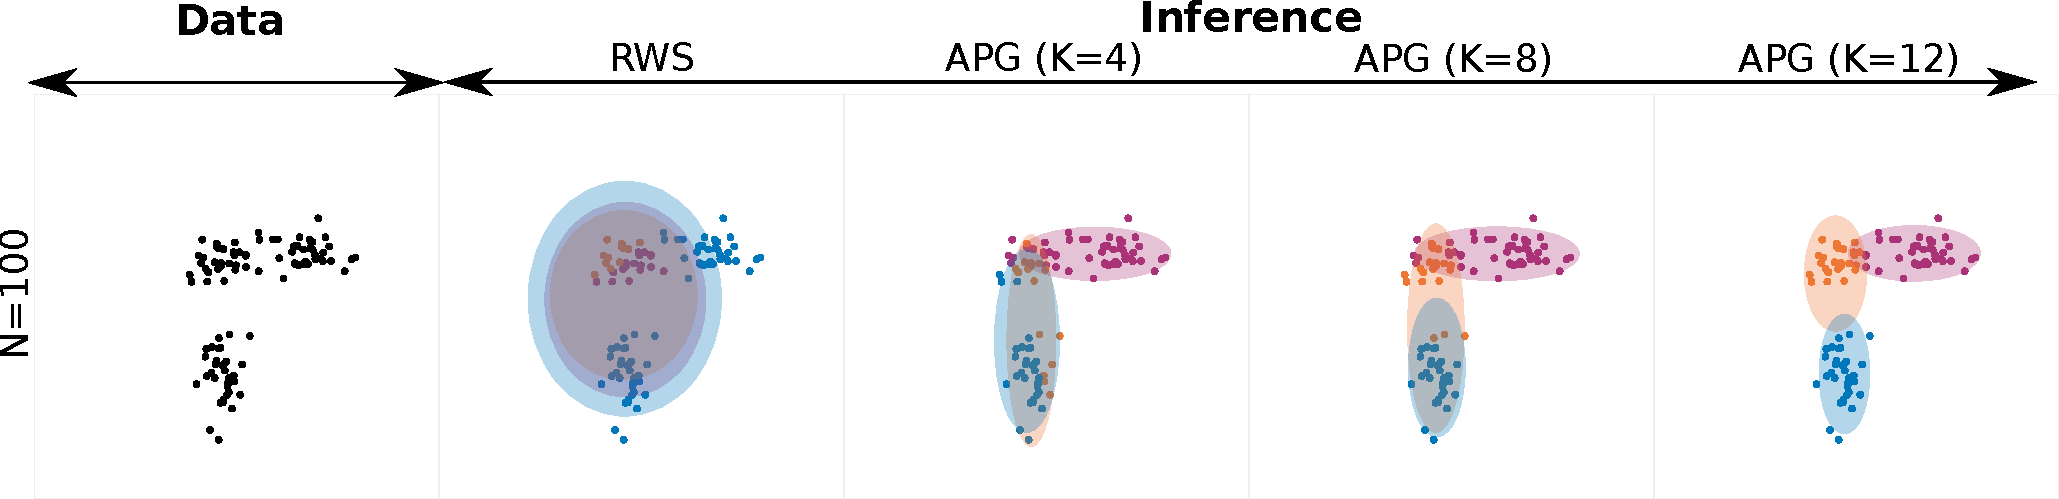
\includegraphics[width=67mm]{figures/gmm_samples_1dataset.pdf}
  \vspace*{-1mm}
  \caption{GMM}
  \label{samples-gmm}
  \vspace{-1ex}
  \end{subfigure}%
  \begin{subfigure}[t]{0.5\textwidth}
  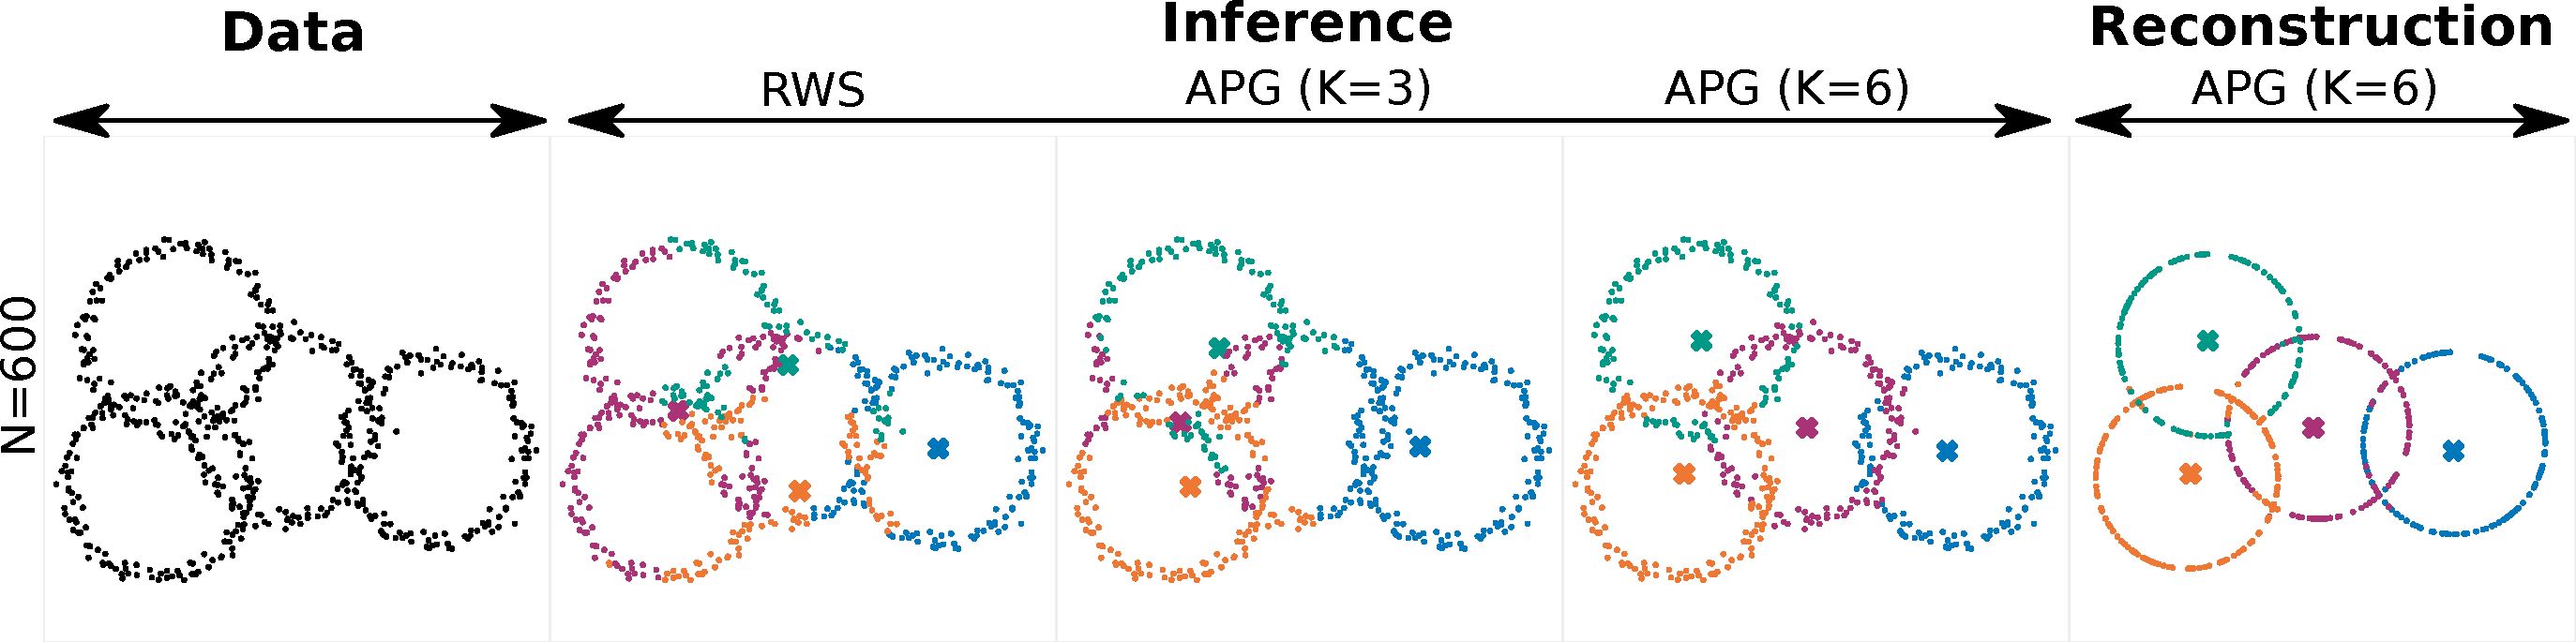
\includegraphics[width=67mm]{figures/dgmm_samples_1dataset.pdf}
  \vspace*{-1mm}
  \caption{DGMM}
  \label{samples-dgmm}
  \vspace{-1ex}
  \end{subfigure}
  \caption{Samples from the GMM and the DGMM. (\textbf{a}) Inference results by RWS, followed by results after 4, 8 and 12 APG updates on one GMM test dataset with $N=100$ data points. (\textbf{b}) Inference results by RWS, followed by results after 3 and 6 APG updates and reconstruction on a DGMM test dataset with $N=600$ data points.}
  \label{samples-mixture}
\end{figure*}
\begin{figure*}[t!]
  \centering
  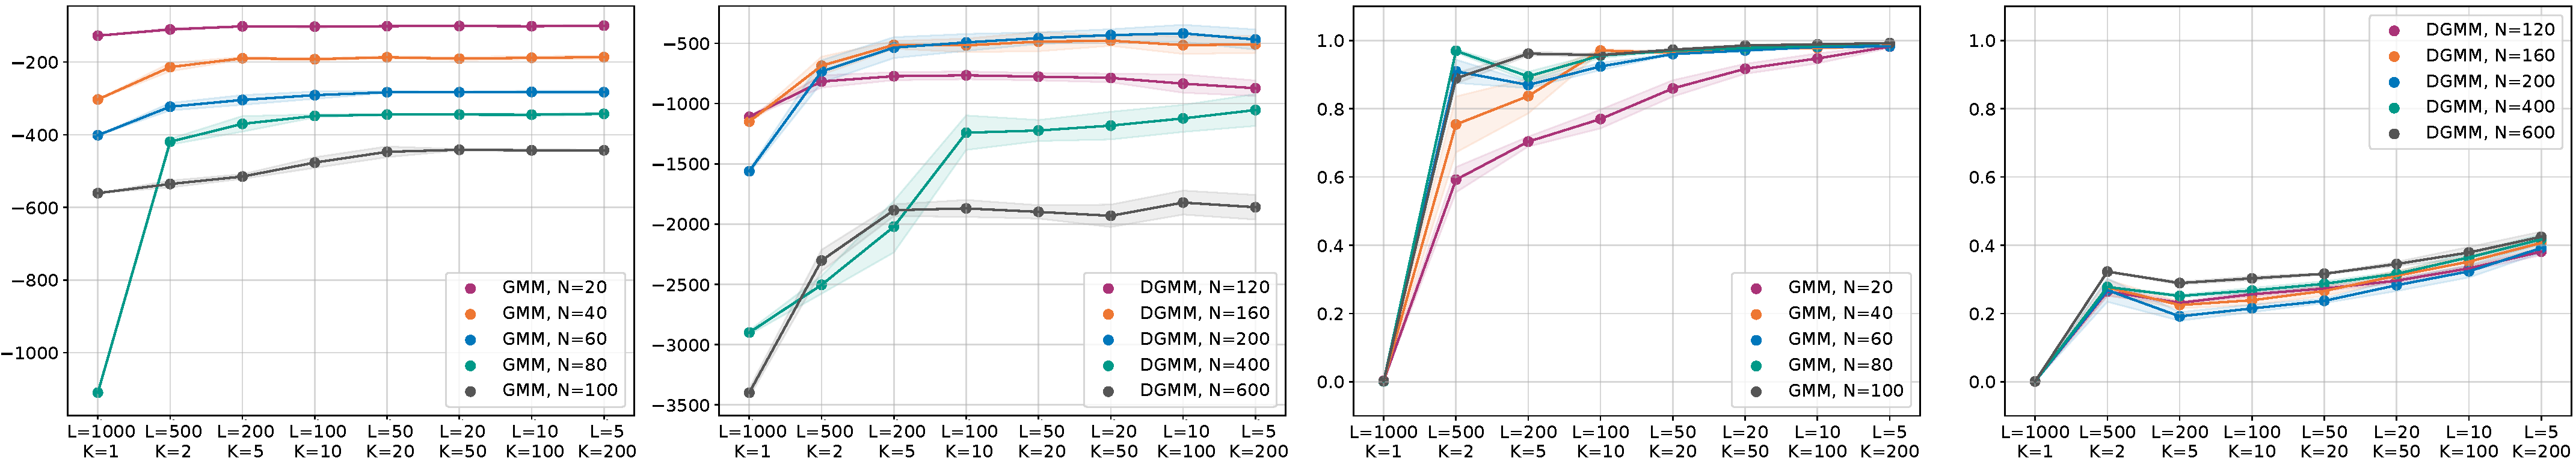
\includegraphics[width=1.0\linewidth]{figures/both-budget-dot-v2.pdf}
  \vspace*{-3mm}
  {\small \hspace{1em}(a) $\log p_\q(x, z)$\hspace{22em}(b) ESS / L}\\
  \caption{APG sampler performance as a function of number of sweeps $K$ for a constant sample budget $K \cdot L = 1000$.}
  \label{fig:budget}
\end{figure*}

\setlength{\tabcolsep}{2pt}
\begin{table*}[t!]
    \centering
    \caption{APG performance in the GMM and DGMM.
    The left column in each table shows the change in log joint distribution, i.e. the difference between the log joint in the baseline and the log joint in other models. We compute the ESS/L metric is computed w.r.t.~different variable blocks. For the GMM we additionally report the inclusive KL (Equation~\ref{eq:variational_objective}) for each block.}
    \begin{subtable}{.4\linewidth}
    \centering
    \caption{GMM}
    \vspace{-0.6em}
    \begin{tabular}{ccc|cccc}
     
    \toprule
        & $\Delta \log p_\q(x, z)$ & 
        \multicolumn{3}{c}{ESS/L} &
        \multicolumn{2}{c}{$\mathrm{KL}(p_\q || q_\f)$}\\
      & & \{$\tau, \mu, c$\} & \{$\tau, \mu$\} & \{$c$\} &\{$\tau, \mu$\}  & \{$c$\} \\
    \midrule
     MLP-RWS & -- & 0.001 & --& -- & -- & --\\
     LSTM-RWS & 202.2 & 0.104 & -- & -- & --
     & -- \\
     APG (K=5) & 198.5 & 0.261 & 0.980 &  0.631 & 0.005 & 0.005
\\
     APG (K=10) & 211.9 & 0.398 & 0.981  & 0.760
     & 0.004 & 0.004
     \\
     APG (K=15) & 215.2 & 0.416 & 0.983 & 0.780 & 0.003 & 0.004\\
    \bottomrule
    \end{tabular}   
    \label{table-gmm}
    \end{subtable}%
    \begin{subtable}{.85\linewidth}
    \centering
    \caption{DGMM}
    \vspace{-0.6em}
    \begin{tabular}{cc|cc}
    \toprule
     $\Delta \log p_\q(x, z)$ & 
         \multicolumn{3}{c}{ESS/L} \\
         & \{$\mu, c, \alpha $\}& \{$\mu$\} & \{$c, \alpha$\}\\
    \midrule
    2538 & 0.001 & -- & -- \\
    -- & 0.001 & -- & --\\
    6201 & 0.002 & 0.013 & 0.422 \\
    6293 & 0.002 & 0.019 & 0.454 \\
    6310 & 0.003 & 0.025 & 0.488 \\
    \bottomrule
    \end{tabular}
    \label{table-dgmm}
    \end{subtable}
    \label{table-both-mm}
\end{table*}
Results on each of these tasks constitute a significant advance relative to the state of the art. Standard VAEs perform poorly at Gaussian mixture modeling tasks, and to our knowledge there are no existing methods that scale to a problem of the complexity of the DGMM for rings. In the context of the unsupervised tracking model, APG easily scales beyond previously reported results for a specialized recurrent architecture \cite{kosiorek2018sequential}. APG is not only is able to scale to models with higher complexity in these settings, but also provides a general framework for performing inference in models with global and local variables, which can be adapted to a variety of model classes with comparative ease.

\subsection{Gaussian Mixture Model}
\label{sec:gmm}
\vspace{-0.5em}
To evaluate whether APG samplers can learn the exact Gibbs updates in conditionally conjugate models, we consider a Gaussian mixture model 
\begin{align*}
    \mu_i, \tau_i \sim \text{NormGamma}(\mu_0, \nu_0, \alpha_0, \beta_0)
    , i &=1,2..,I \\
    c_n \sim \mathrm{Cat}(\pi), 
    x_n | c_n\!=\!i \sim \text{Norm}(\mu_i, 1 / \tau_i)
    ,n &=1,2,..,N
\end{align*}
In this model, the global variables $z^\textsc{g} = \{\mu_{1:I}, \tau_{1:I}\}$ are the mean an precision for each mixture component, whereas the local variables are the cluster assignments $z^\textsc{l} = \{c_{1:N}\}$. Conditioned on cluster assignments, the Gaussian likelihood $p(\x_{1:N} \mid z_{1:N}, \mu_{1:I}, \tau_{1:I})$ is conjugate to a normal-gamma prior $p(\mu_{1:I}, \tau_{1:I})$ with sufficient statistics $T(x_n, c_n)$ 
\begin{align*}
    \Big\{\mathrm{I}[c_n \!=\! i], 
        ~\mathrm{I}[c_n \!=\! i] \: x_n, 
        ~\mathrm{I}[c_n \!=\! i] \: x_n^2 
        ~\Big\vert~ i \!=\! 1,2,\dots,I 
    \Big\}
    ,
\end{align*}
where $\mathrm{I}[z_n \!=\! i]$ is an indicator function that evaluates to 1 if the equality holds, and 0 otherwise.

We employ a variational distribution that updates the global variables $q_\f(\mu, \tau \mid x, c)$ and the local variables $q_\f(c \mid x, \mu, \tau)$, using point-wise neural sufficient statistics modeled after the ones in the analytical updates (see Appendix \ref{appendix:architecture} for architecture details).

We train our models on 20,000 datasets with $I = 3$ clusters and $N = 60$ data points with fixed hyperparameters ($\mu_0 = 0$, $\nu_0 = 0.3$, $\alpha_0 = 2$, $\beta_0 = 2$). We use $20$ GMM datasets per batch, $K=10$ sweeps, $L=10$ particles, and Adam ($\mathrm{lr} = 10^{-4}, \beta_1 = 0.9, \beta_2 = 0.99$) for 200,000 iterations.

We compare the APG sampler to samples from a standard encoder with MLP and LSTM architectures,  which is trained using reweighted wake-sleep (RWS). Both architectures are parameterized using the same neural sufficient statistics as the APG sampler.

Figure \ref{samples-gmm} shows sequences of single samples from the variational distribution, where the first sample is drawn using RWS. Even when using a parameterization that employs neural sufficient statistics, the RWS encoder fails to propose reasonable clusters, whereas the APG sampler typically converges within 12 iterations across a range of dataset sizes.

Furthermore, we would like to quantify how similar learned proposals $q_\f(z_b \mid x, z_{-b})$ are to the conditional posteriors $p_\q(z_b \mid x, z_{-b})$. With the case of GMM where the exact conditional posterior is tractable, we verify the convergence of the learned proposals by computing the inclusive KL divergence $\mathcal{K}_b(\f)$ defined in equation ~\ref{eq:variational_objective} (see Table \ref{table-gmm}). We can see that the APG samplers of the both $\{\tau, \mu\}$ and $\{c\}$ converge to the true conditional posterior.


% \begin{figure}[t!]
%   \centering
%   {\small \hspace{1em}\textsf{\textbf{GMM}}\hspace{10em}\textsf{\textbf{DGMM}}}\\
%   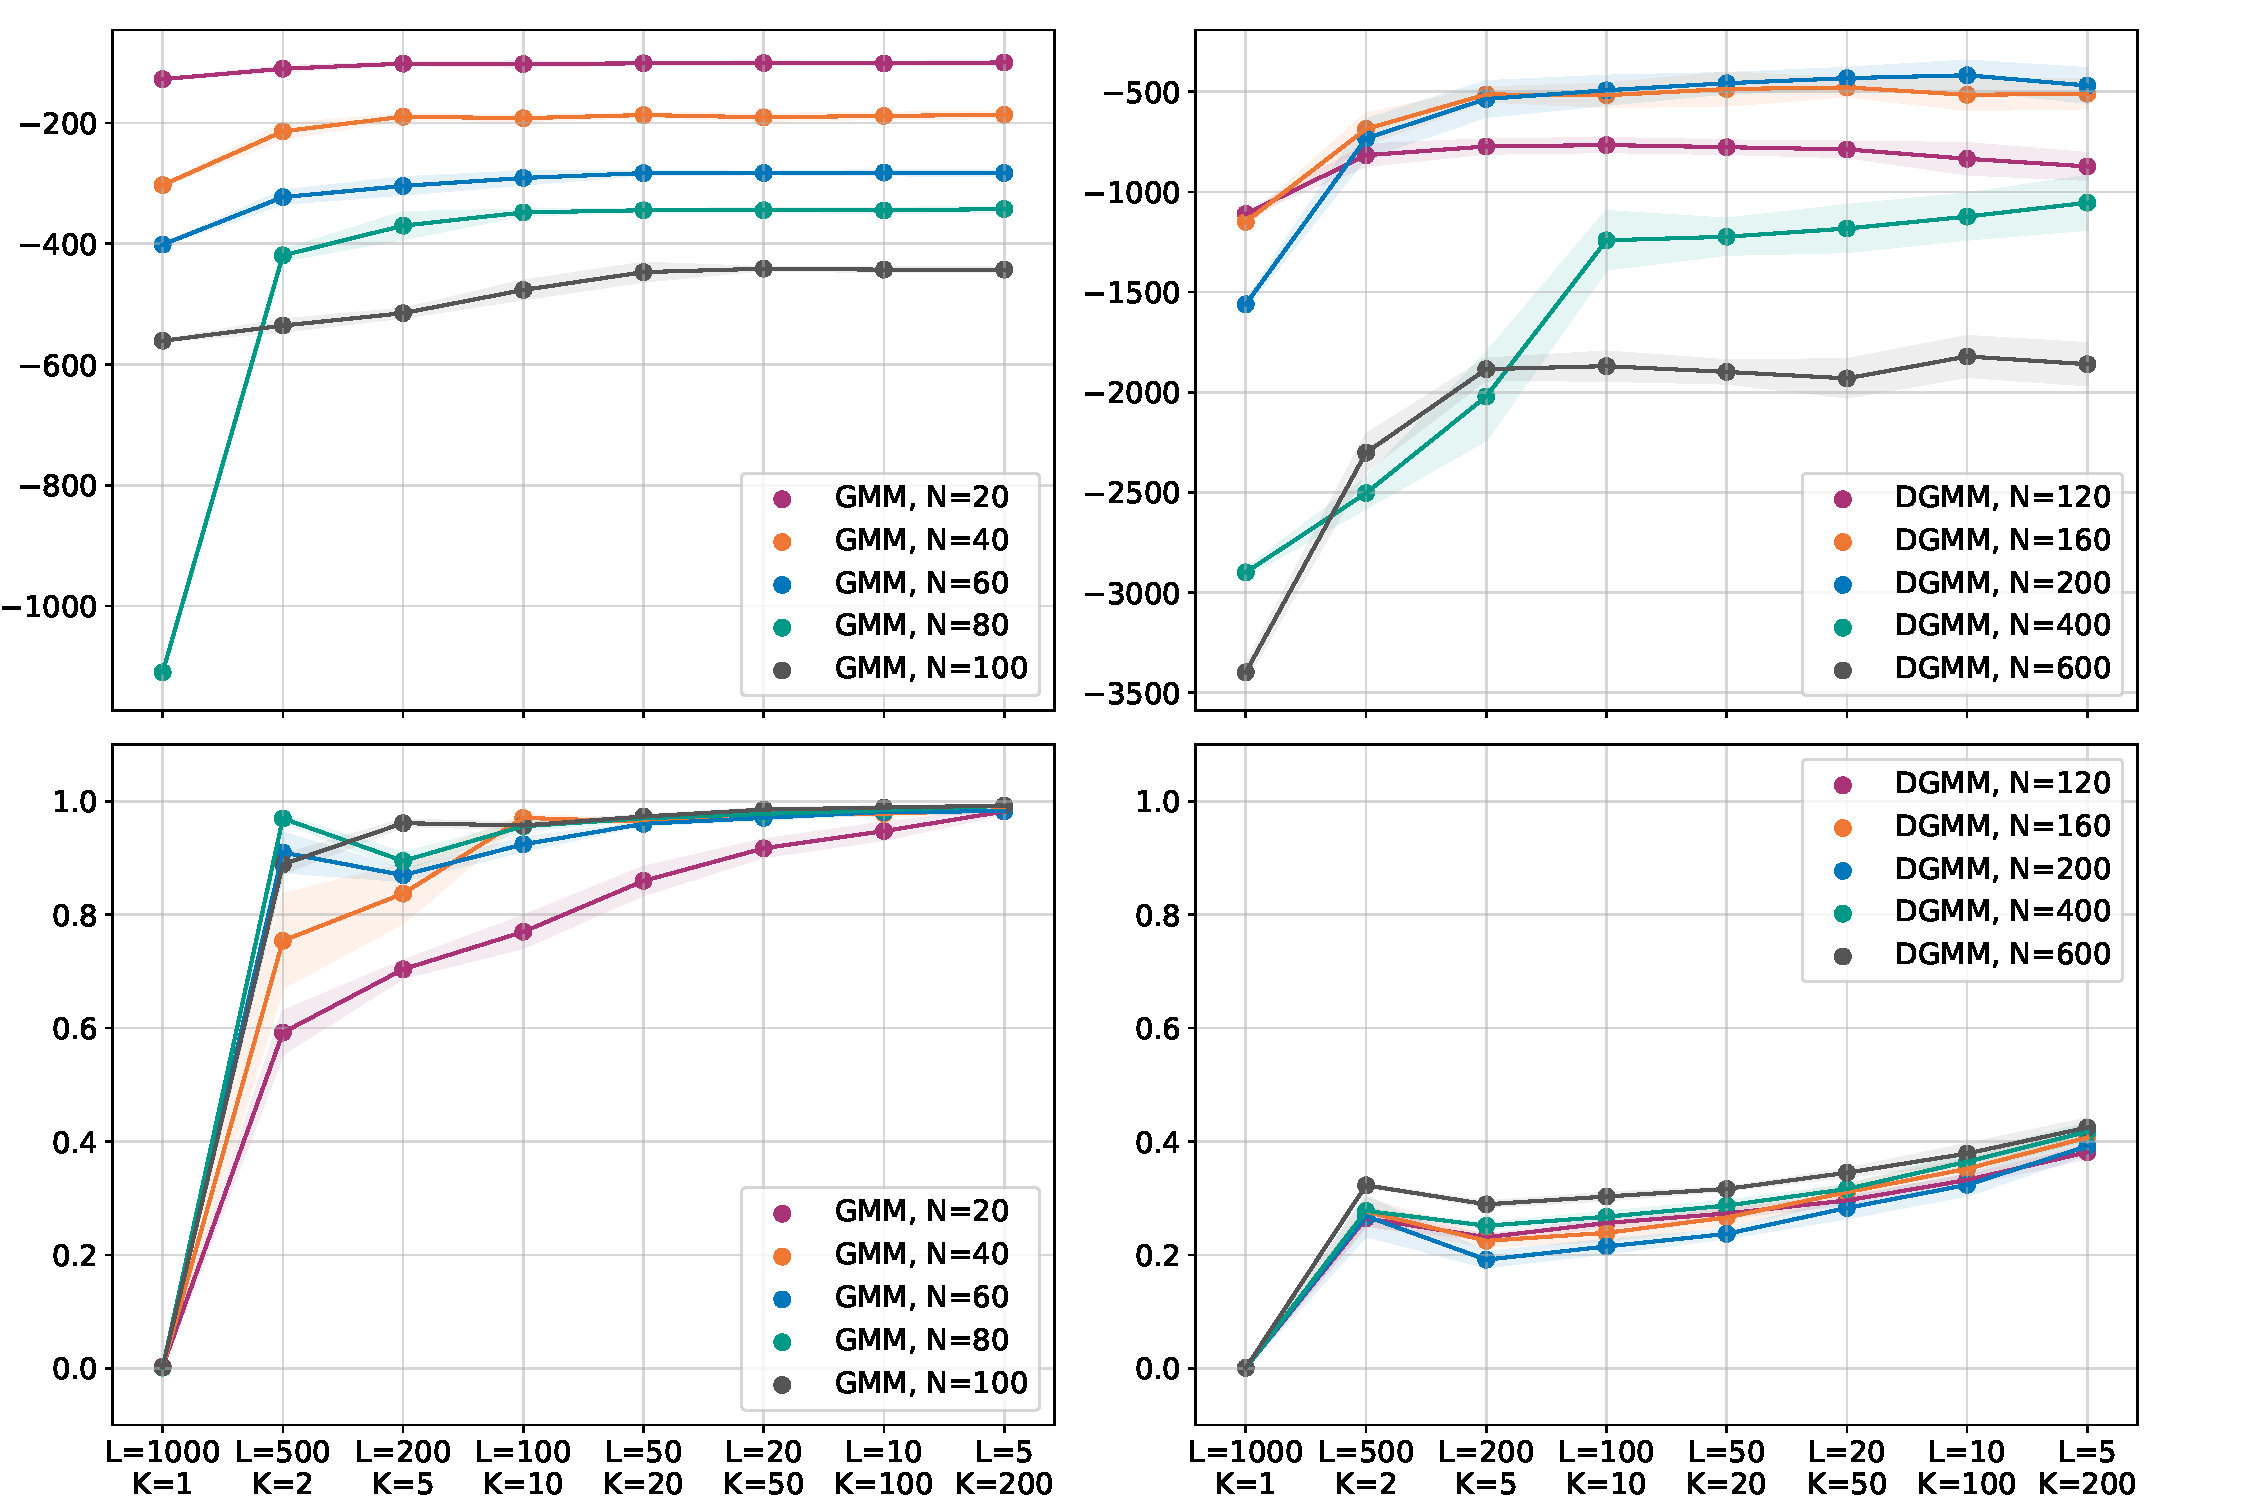
\includegraphics[width=1.0\linewidth]{figures/both-budget-dot.pdf}
% %   \vspace*{-3mm}
%   \caption{APG sampler performance as a function of number of sweeps $K$ for a constant sample budget $K \cdot L = 1000$.\\ \textbf{Top}: Log joint $\log p_\q(\x ,\z)$. \textbf{Bottom}: ESS / L.}
%   \label{fig:budget}
% \end{figure}

\subsection{Deep Generative Mixture Model}
We next consider the task of training a deep generative model $p_\q(\x, \z)$ is jointly with the APG sampler. Our dataset consists of ring-shaped clusters. The true generative model (which we assume is unknown) takes the form
\begin{align*}
    \mu_i \sim \text{Norm}(0, 
    \sigma_0^2 I), 
    \qquad i = 1, 2, ..., I \\
    c_n \sim \mathrm{Disc}(\pi), \quad \alpha_n \sim \mathrm{Unif}[0, 2\pi], \\
    x_n | c_n=i \sim \text{Norm}(g_\q(\alpha_n) + \mu_i, \Sigma_\epsilon).
\end{align*}
Here $\mu_i$ is center of the $i$th ring. Given a cluster assignment $c_n$ and an angle $\alpha_n$ we define a position on a ring, from which We sample a data point $x_n$ with 2D Gaussian noise.

\begin{figure*}[!h]
  \centering
%   \begin{subfigure}[t]{1.0\textwidth}
%   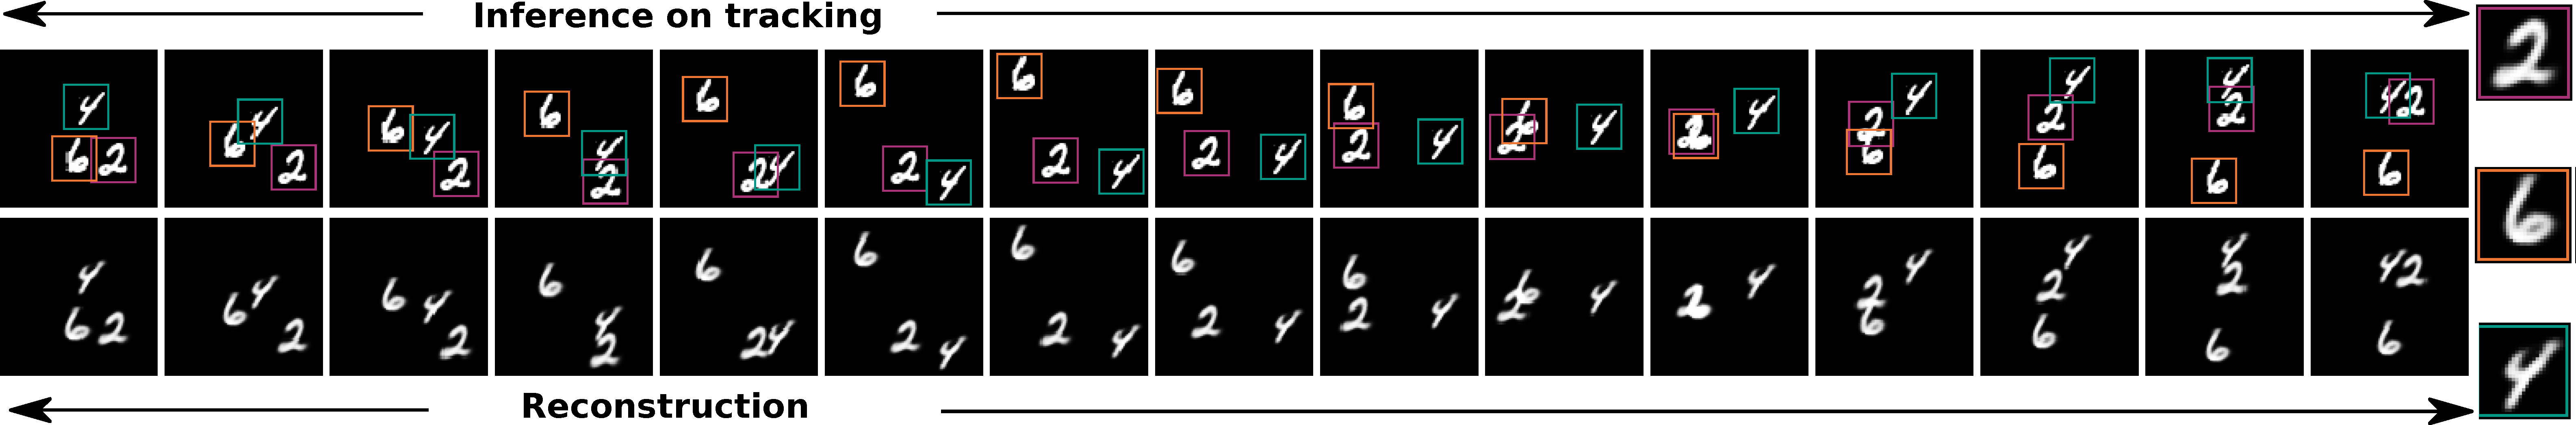
\includegraphics[width=1.0\textwidth]{figures/bmnist-3digits-samples.pdf}
% %   \vspace*{-5mm}
% %   \caption{3 digits.}
%   \end{subfigure}
%   %%%%%%%%%%%
%   \begin{subfigure}[t]{1.0\textwidth}
%   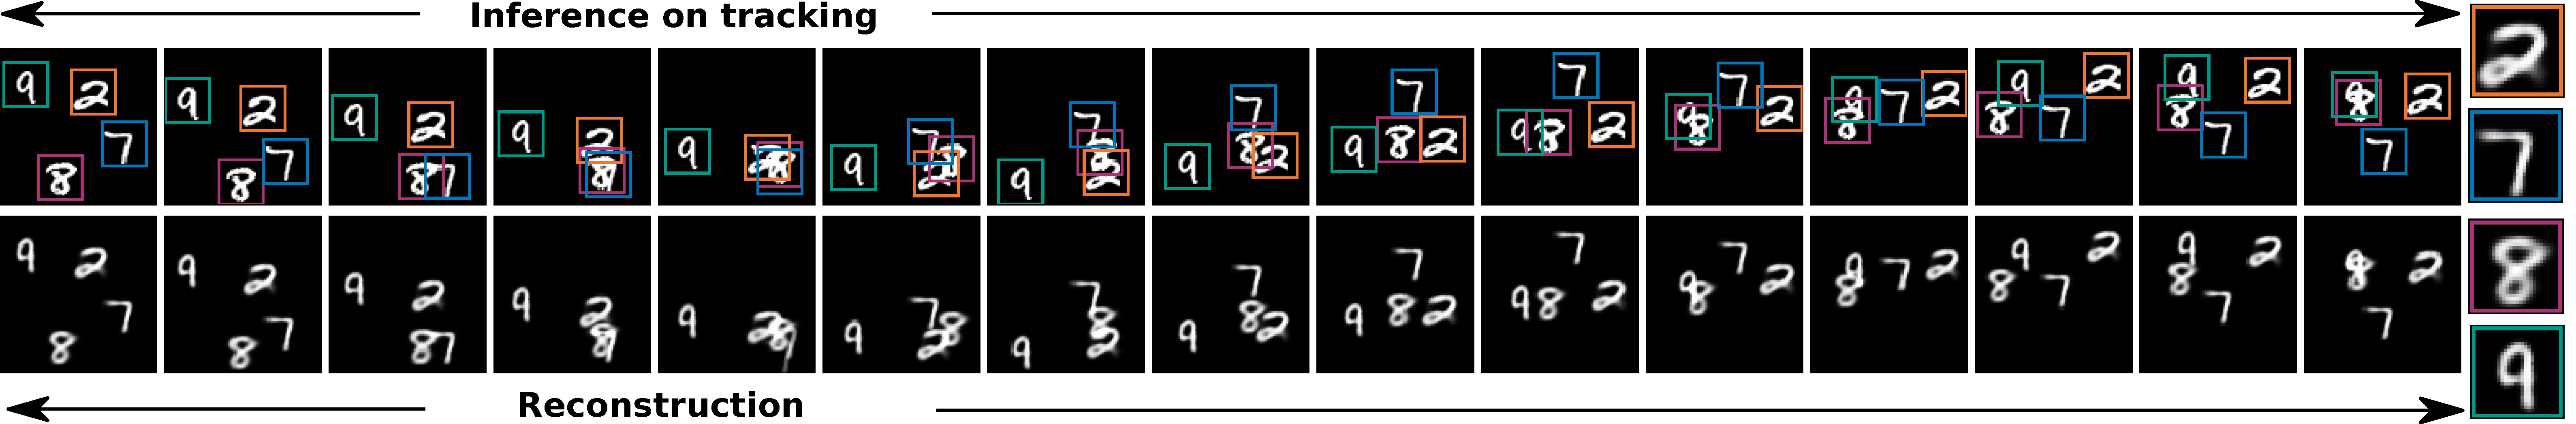
\includegraphics[width=1.0\textwidth]{figures/bmnist-4digits-samples.pdf}
% %   \vspace*{-5mm}
% %   \caption{4 digits.}
%   \end{subfigure}
%   %%%%%%%%%%%
  \begin{subfigure}[t]{1.0\textwidth}
  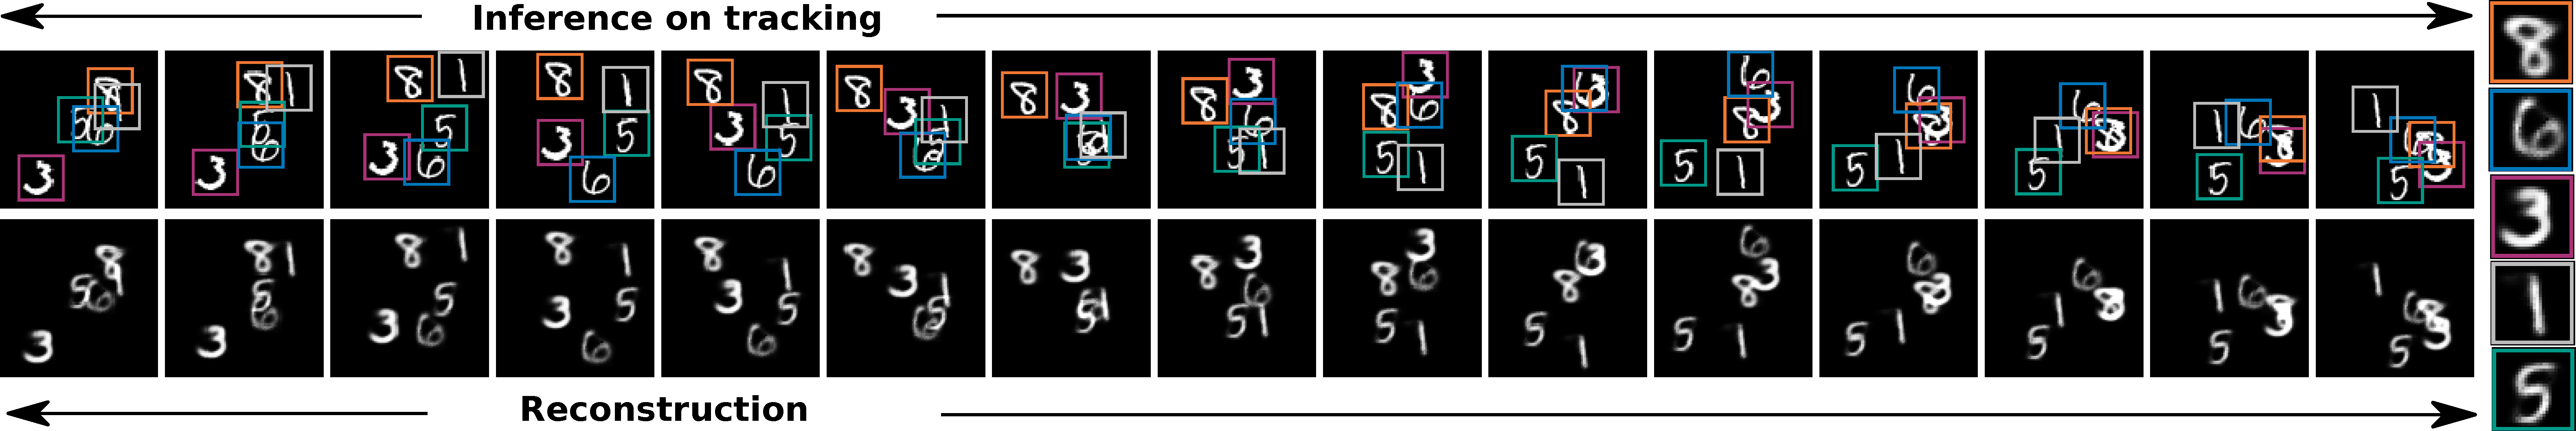
\includegraphics[width=1.0\textwidth]{figures/bmnist-5digits-samples.pdf}
%   \vspace*{-5mm}
%   \caption{5 digits.}
  \end{subfigure}
  \caption{Inferred digit trajectories and reconstructions for $D = 5$ digits for $T = 15$ for a model trained on $D = 3$ and $T = 10$.}
  \label{mnist-qualitative}
\end{figure*}

We train our model on 20,000 datasets with $N = 200$ data points and $I = 4$ clusters with fixed hyperparameters ($\sigma_0 = 3.5$, $\Sigma_{\epsilon} = 0.2$). We use $20$ datasets per batch, $K=10$ sweeps, $L=10$ particles, and Adam ($\mathrm{lr} = 10^{-4}, \beta_1 = 0.9, \beta_2 = 0.99$) for 200,000 iterations (see Appendix \ref{appendix:architecture} for architecture details).

Once again, we compare the APG sampler with the encoders using RWS. Figure~\ref{samples-dgmm} shows individual samples analogous to the ones in Figure~\ref{samples-gmm}. The APG sampler scales to a large range of number of variables, whereas a standard encoder trained using RWS fails to produce reasonable proposals.

\subsection{Sample Quality Evaluation}
In both mixture models, we compute the log-joint distribution $\log p_\q(\x, z)$ (see Table \ref{table-both-mm}) as a function of sweep iteration to measure the convergence and the effective sample size (see Table \ref{table-both-mm}) to assess proposal quality
\begin{align}
\label{ess-eq}
    \frac{\text{ESS}}{L} 
    = 
    \frac{(\sum_{l=1}^L w^{k,l})^2}
         {L \sum_{l=1}^L (w^{k,l})^2}
    .
\end{align}


\textbf{Log joint} $\log p_\q(\x, z)$. Because the marginal $q_\f(z^k | x)$ is intractable, it is difficult to compute an lower bound or upper bound at each sweep. Here we compute the log joint in each test dataset for both the APG sampler with different number of sweeps and the RWS baselines and report the differences on average to see how much more is achieved by the APG sampler. In both models, the APG sampler gains a higher log joint compared with the encoder trained by RWS.

\textbf{ESS}. One advantage of the APG sampler that it decomposes a high dimensional sampling problem into a sequence of lower dimensional sampling problems. To show that, we compute the ESS when 1) we resample only after one sweep and 2) we resample after each block update. WE can see that the granular sampling strategy significantly improves the ESS in both cases.

\subsection{Fixed Computation Budget Analysis}
As a mean of comparing the performance of APG samplers for varying numbers of sweeps $K$, we perform an experiment in which the computation budget is fixed at $K \cdot L = 1000$ samples. Figure~\ref{fig:budget} shows $\log p_\theta(x, z)$ and ESS/L. The shaded area denotes the standard deviation over 10 runs that each comprise 5 datasets that were chosen at random. We can see that it in general, it is more effective to perform more APG sweeps $K$ with a smaller number of particles $L$, that it is to increase the particle budget. 

\subsection{Time Series Model -- Bouncing MNIST}
Finally, we apply the APG sampler to a time series model that is trained with short timescales, and evaluate its performance with longer timescales and larger numbers of latent variables.
The data $x_{1:T}$ is a sequence of images of $D$ moving MNIST digits.
Our generative model consists of global variables $\z_{1:D}^{\mathrm{what}}$ corresponding to digit latent variables and local variables $\z_{1:D, 1:T}^{\mathrm{where}}$ corresponding to the digit trajectories.
The deep generative model is a state space model that factorizes across digits of the form
\begin{align*}
    z^{\mathrm{what}}_{d} 
    &\sim 
    \text{Norm}(0, I), 
    \,\,\, 
    z^{\mathrm{where}}_{d, 1} \sim \text{Norm}(0, I), 
    \\
    z^{\mathrm{where}}_{d, t} 
    %| z^{\mathrm{where}}_{d, t - 1} 
    &\sim 
    \text{Norm}(z^{\mathrm{where}}_{d, t - 1}, \sigma^2_0 I) 
    \\
    x_t 
    %| z^\mathrm{where}_{d,t}, z^\mathrm{what}_d 
    &\sim
    \mathrm{Bern}
    \Big(
        \sigma
        \Big(
            \sum_{d} \mathrm{ST}
            \big(
                \mu_\theta(\z^{\mathrm{what}}_d), 
                z^{\mathrm{where}}_{d, t}
            \big)
        \Big)
    \Big)
\end{align*}
Here, ST is a spatial transformer \cite{jaderberg2015spatial} that maps the output of a feedforward decoder $\mu_\q$ that maps logits for a 28$\times$28 MNIST image onto a 96$\times$96 canvas based on the location variable $z^{\mathrm{where}}_{d, t}$. 

Our amortized Gibbs updates employ $T + 1$ blocks $(z_{1:D}^{\mathrm{what}}, z_{1:D, 1}^{\mathrm{where}}, z_{1:D, 2}^{\mathrm{where}}, \dotsc, z_{1:D, T}^{\mathrm{where}})$.
Empirically this works better than splitting the latent variables into global and local variables, since resampling at each time step $t$ helps disentangle the digit locations if they overlap.

We train our model on 60000 bouncing MNIST sequences, each of which contains $D=3$ digits and $T=10$ frame images. We use $10$ sequences per batch, $K=5$ sweeps, $L=10$ particles, and Adam ($\mathrm{lr} = 10^{-4}, \beta_1 = 0.9, \beta_2 = 0.99$) for 200,000 iterations (see Appendix \ref{appendix:architecture} for architecture details).

We show that APG sampler can scale to larger number of variables by testing the model on datasets with $T\in \{20, 100\}$ time steps  and $D \in \{3, 4, 5\}$ digits. Figure~\ref{mnist-qualitative} shows the inference and reconstruction using single samples from the variational distribution. (plots are truncated by the first $15$ time steps due to limited space, see Appendix \ref{appendix:full-recons} for more examples with full time steps). 
Qualitatively, we see that the digit trajectories $\z_{1:D, 1:T}^{\mathrm{where}}$ and latent variables $\z_{1:D}^{\mathrm{what}}$ are inferred well.
In Figure~\ref{plot-mse-bmnist}, we show the mean squared error between the video and its reconstruction for different $T$ and $D$.
The results confirm that performance improves with increasing number of Gibbs sweeps $K$.
In certain cases, a larger number of time points $T$ in fact improves convergence as a function of the number of sweeps $K$.

\begin{figure}[!t]
    \centering
    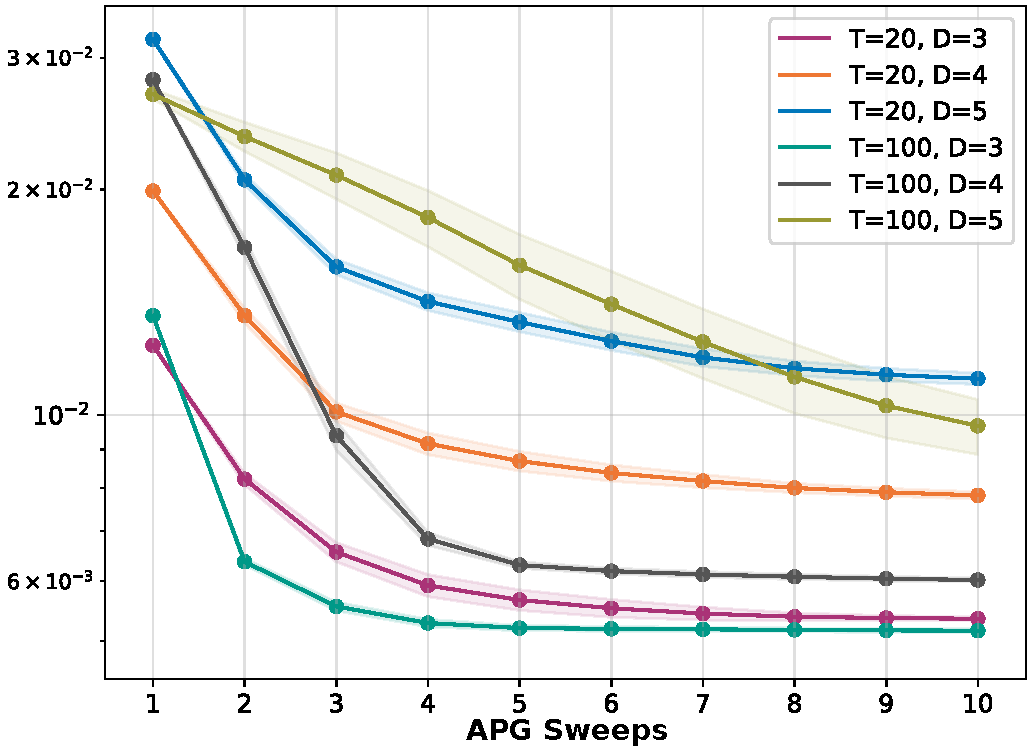
\includegraphics[width=0.5\columnwidth]{figures/bmnist-mse.pdf}
    \caption{Mean squared error between video frames and reconstructions as a function of the number of APG sweeps. }
    \label{plot-mse-bmnist}
\end{figure}

\section{Conclusion}

% We developed amortized Gibbs samplers that iterate between updates to global and local variables using neural proposals. These methods offer a path towards designing variational approximations to intractable posteriors in structured deep generative models. APG samplers have particular strengths in problems with global variables, but more generally make it possible to design amortized approaches that exploit conditional independence. This decomposes high-dimensional sampling problems into a sequence of lower-dimensional problems, hereby greatly reducing estimator variance. Moreover, our parameterization in terms of neural sufficient statistics makes it comparatively easy to design models that will generalize to datasets that vary in size. 

One of the challenges in amortized inference for deep generative models is learning high-quality proposals for models with a structured prior over a high-dimensional set of latent variables. These priors arise naturally when, rather than encoding a single data point (e.g.~an image), we wish to encode a dataset (e.g.~a sequence of images). 
Even for apparently simple problems, such as inferring the cluster parameters and assignments in a mixture model, standard encoders often fail to produce good samples. One of the reasons for this is that it is fundamentally difficult to jointly generate proposals for a high-dimensional set of latent variables.

APG samplers are very general, and offer a path towards the development of deep generative models that incorporate structured priors to provide meaningful inductive biases in settings where we have little or no supervision. These methods have particular strengths in problems with global variables, but more generally make it possible to design amortized approaches that exploit conditional independence. Moreover, our parameterization in terms of neural sufficient statistics makes it comparatively easy to design models that scale to much larger number of latent variables and thus generalize to datasets that vary in size. 

Immediate lines of future work are to compare the approach in this paper, which learns kernels that leave the target density invariant, with approaches that perform annealing, in which the learned kernels are assymmetric in the sense that they gradually transform the initial encoder distribution to the target density. 

\section{Acknowledgements}

This work was supported by the Intel Corporation, NSF award 1835309, the DARPA LwLL program, and startup funds from Northeastern University. Tuan Anh Le was supported by AFOSR award FA9550-18-S-0003.


\bibliographystyle{acm-reference-format}
\bibliography{references}
\newpage
\section{Appendices}
\subsection{SMC Sampler Algorithm}
\label{appendix:smc-alg}
\begin{algorithm}[!h]
\setstretch{1.2}
  \caption{SMC sampler}
  \label{alg:smcs}
\begin{algorithmic}[1]
    \small
    \For{$l = 1$ \textbf{to} $L$}
        \State $z^{1,l} \sim q^1(\cdot)$\Comment{Propose}
        \State $w^{1,l} = \frac{\gamma^1(z^{1,l})}{q^1(z^{1,l})}$\Comment{Weigh}
    \EndFor
    \For{$k = 2$ \textbf{to} $K$}
      \State$z^{k-1,1:L}, w^{k-1,1:L}=\textsc{resample}(z^{k-1,1:L}, w^{k-1,1:L})$
    %   \State$\{z^{k-1,l}, w^{k-1,l}\}_{l=1}^L=\textsc{resample}(\{z^{k-1,l}, w^{k-1,l}\}_{l=1}^L)$

      \For{$l = 1$ \textbf{to} $L$}
          \State $z^{k,l} \sim q^k(\cdot \mid z^{k-1,l})$\Comment{Propose}\label{line:apg-propose}
          \State $w^{k,l} = \frac{\gamma^k(z^{k,l}) r^{k-1}(z^{k-1,l} \mid z^{k,l})}{\gamma^{k-1}(z^{k-1,l}) q^k(z^{k,l} \mid z^{k-1,l})}w^{k-1,l}$\Comment{Weigh}
      \EndFor
    \EndFor
\end{algorithmic}
\end{algorithm}

\subsection{Resampling Algorithm}
\label{appendix:resample-alg}
\begin{algorithm}[!h]
    \setstretch{1.2}
  \caption{\textsc{resample}}
  \label{alg:resample}
\begin{algorithmic}[1]
\small
  \State \textbf{Input:} $z^{\:1:L}, w^{\:1:L}$
  \State \textbf{Output:} $z'^{\:1:L}, w'^{\:1:L}$
  \For {$i = 1$ \textbf{to} $L$}
    \State $a^i \sim \mathrm{Disc}(\{w^l / \sum_{l' = 1}^L w^{l'}\}_{l=1}^L)$\Comment{Index Selection} 
    % \State $P(a^i = l) = w^l / \sum_{l' = 1}^L w^{l'}$
    \State Set $ z'^{\:i} = z^{a^i}$
    \State Set $ w'^{\:i} = \frac{1}{L} \sum_{l = 1}^L w^l$\Comment{Re-Weigh}
    \EndFor
  \State \textbf{Return} $z'^{\:1:L}, w'^{\:1:L}$
\end{algorithmic}
\end{algorithm}

\subsection{Gradient of the generative model}% $p_\q(x \mid z)$}
\label{appendix:grad-theta}
This is actually a known (although indeed not obvious) identity. Briefly, we can express the expected gradient of the log joint as
\begin{align*}
    \mathbb{E}_{p_\q(\z | \x)} 
    \left[
    \nabla_\q \log p_\q(\x, \z)
    \right]
    \mathbb{E}_{p_\q(\z | \x)} 
    \left[
    \nabla_\q \log p_\q(\x) + \nabla_\q \log p_\q(\z | \x)
    \right]
    \mathbb{E}_{p_\q(\z | \x)} 
    \left[
    \nabla_\q \log p_\q(\x) 
    \right]
    \nabla_\q \log p_\q(\x)
\end{align*}
Here we make use of a standard identity that is also used in, e.g., likelihood-ratio estimators
\begin{align*}
\mathbb{E}_{p_\q(\z | \x)}
\left[
    \nabla_\q \log p_\q(\z | \x)
\right] 
=
\int p_\q(\z | \x) \nabla_\q \log p_\q(\z | \x) \: dz
=
\int \nabla_\q p_\q(\z | \x) \: dz
=
\nabla_\q \int p_\q(\z | \x) \: dz
=
\nabla_\q 1
= 
0
\end{align*}
Therefore, we have the the following equality
\begin{align*}
\nabla_\q \log p_\q(\x) 
= 
\mathbb{E}_{p_\q(\z | \x)} 
\left[
\nabla_\q \log p_\q(\x, \z)
\right].
\end{align*}
which is Equation ~\ref{eq:grad-theta}. As a result, we can then use self-normalized importance sampling to approximate     $\mathbb{E}_{p_\q(\z | \x)} \left[\nabla_\q \log p_\q(\x, \z) \right]$.

\subsection{Importance weights in sequential importance sampling}
\label{appendix:sis-weight}
At step $k=1$, we use exactly the standard importance sampler, thus it is obvious that the following is a valid importance weight
\begin{align*}
    w^1 = \frac{\gamma^1(z^1)}{q^1(z^1)}.
\end{align*}
When step $k>2$, we are going to prove that the importance weight relative to the intermediate densities has the form
\begin{align}
    \label{appendix:eq:sis-weight}
    w^k
    = 
    \frac{\gamma^k(z^{1:k})}
         {q^1(z^1) \prod_{k'=2}^k q^{k'}(z^{k'} \mid z^{1:k'-1})}.
\end{align}

At step $k=2$, the importance weight is defined as 
\begin{align*}
    w^k 
    &= 
    v^{2} \: w^1
    \: =
    \frac{\gamma^2(z^{1:2})}{\gamma^{1}(z^{1})\:q^2(z^2 \mid z^{1})} \frac{\gamma^1(z^1)}{q^1(z^1)}
    \: = \frac{\gamma^2(z^{1:2})}{q^1(z^1) \: q^2(z^2 \mid z^{1})}.
\end{align*}
which is exactly that form. Now we prove weights in future steps by induction. At step $k\geq 2$, assume the weight has the form in Equation~\ref{appendix:eq:sis-weight}, i.e.
\begin{align*}
    w^k
    = 
    \frac{\gamma^k(z^{1:k})}
         {q^1(z^1) \prod_{k'=2}^k q^{k'}(z^{k'} \mid z^{1:k'-1})}.    
\end{align*}
, then at step $k+1$, the importance weight is the product of incremental weight and incoming weight 
\begin{align*}
    w^{k+1}
    =
    v^{k+1} \: w^k
    =
    \frac{\gamma^{k+1}(z^{1:k+1})}{\gamma^{k}(z^{1:k})\:q^{k+1}(z^{k+1} \mid z^{1:k})}
    \frac{\gamma^k(z^{1:k})}
         {q^1(z^1) \prod_{k'=2}^k q^{k'}(z^{k'} \mid z^{1:k'-1})}
    =
    \frac{\gamma^{k+1}(z^{1:k+1})}{q^1(z^1) \prod_{k'=2}^{k+1} q^{k'}(z^{k'} \mid z^{1:k'-1})}
    .    
\end{align*}
Thus the importance weight $w^k$ has the form of Equation~\ref{appendix:eq:sis-weight} at each step $k>2$ in sequential importance sampling.
\subsection{Derivation of Posterior Invariance}
\label{appendix:posterior-invariance}
We can see that individual block updates leave the posterior invariant by proposing variables $\z^k_{\preceq b}$ from a partial kernel $\kappa(\z^k_{\preceq b} \mid x, \z^{k-1})$ and then marginalize over the corresponding variables from the previous step $\z^{k-1}_{\preceq b}$,
\begin{align*}
    \int 
    dz^{k-1}_{\preceq b} 
    \:
    p_\q(\z^{k-1} \mid \x) 
    \: 
    \kappa(\z^k_{\preceq b} \mid x, \z^{k-1}) 
    %\\
    %&= 
    &=
    \int 
    dz^{k-1}_{\preceq b} 
    \:
    p_\q(\z^{k-1} \mid \x) 
    \: 
    \int dz^k_{\succ b}
    \:
    \kappa(\z^k \mid x, \z^{k-1})
    \\
    &= 
    \int 
    dz^{k-1}_{\preceq b} 
    \: 
    p_\q(\z^{k-1} \mid x)
    \prod_{m=1}^b p_\q(\z^k_m \mid \x, \z^{k}_{\prec m}, \z^{k-1}_{\succ m})
    \\
    &=
    \int 
    dz^{k-1}_{\preceq b} 
    \: 
    p_\q(\z^{k-1} \mid \x)
    p_\q(\z^k_{\preceq b} \mid \x, \z^{k-1}_{\succ 1})
    \\
    %&=
    %\int d\z^{k-1}_{\preceq b} 
    %\: p_\q(\z^k_{\preceq b}, \z^{k-1} \mid \x)\\
    &=
    p_\q(\z^k_{\preceq b}\:, \: \z^{k-1}_{\succ b} \mid \x)
    .
\end{align*}

\subsection{Proof of the amortized population Gibbs algorithm}
\label{appendix:proof-algo}

Here, we provide an alternative proof of correctness of the APG algorithm given in Algorithm~\ref{alg:amortized-gibbs}, based on the construction of proper weights~\cite{naesseth2015nested} which was introduced after SMC samplers~\cite{delmoral2006sequential}.
We first introduce proper weights, and then present several operations that preserve the proper weighting property and finally we apply these properties in proving correctness of APG.

\subsubsection{Proper weights}

\begin{definition}[Proper weights]
    Given an unnormalized density $\tilde p(z)$, with corresponding normalizing constant $Z_p := \int \tilde p(z) \,\mathrm dz$ and normalized density $p \equiv \tilde p / Z_p$, the random variables $z, w \sim P(z, w)$ are properly weighted with respect to $\tilde p(z)$ if and only if for any measurable function $f$
    \begin{align}
    \label{eq:pw}
    \E_{P(z, w)}\left[w f(z)\right] = Z_p \E_{p(z)}[f(z)]. 
    \end{align}
    We will also denote this as
    \begin{align*}
        z, w \pw \tilde p.
    \end{align*}
\end{definition}

\paragraph{Using proper weights.}
Given independent samples $z^l, w^l \sim P$, we can estimate $Z_p$ by setting $f \equiv 1$:
\begin{align*}
    Z_p \approx \frac{1}{L} \sum_{l = 1}^L w^l.
\end{align*}
This estimator is unbiased because it is a Monte Carlo estimator of the left hand side of \eqref{eq:pw}.
We can also estimate $\E_{p(z)}[f(z)]$ as
\begin{align*}
    \E_{p(z)}[f(z)] \approx \frac{\frac{1}{L} \sum_{l = 1}^L w^l f(z^l)}{\frac{1}{L} \sum_{l = 1}^L w^l}.
\end{align*}
While the numerator and the denominator are unbiased estimators of $Z_p \E_{p(z)}[f(z)]$ and $Z_p$ respectively, their fraction is biased.
We often write this estimator as
\begin{align}
    \E_{p(z)}[f(z)] \approx \sum_{l = 1}^L \bar w^l f(z^l), \label{eq:pw-estimation}
\end{align}
where $\bar w^l := w^l / \sum_{l' = 1}^L w^{l'}$ is the normalized weight.

\subsubsection{Operations that preserve proper weights}


\begin{proposition}[Nested importance sampling]
    Adapted from \cite[Algorithm 1]{naesseth2015nested}.
    Given unnormalized densities $\tilde q(z), \tilde p(z)$ with the normalizing constants $Z_q, Z_p$ and normalized densities $q(z), p(z)$, if 
    \begin{align}
        z, w \pw \tilde q, \label{eq:1}
    \end{align}
    then
    \begin{align*}
        z, \frac{w\tilde p(z)}{\tilde q(z)} \pw \tilde p.
    \end{align*}
\end{proposition}
\begin{proof}
    First define the distribution of $z, w$ as $Q$.
    For measurable $f(z)$
    \begin{align*}
        \E_{Q(z, w)}\left[\frac{w\tilde p(z)}{\tilde q(z)} f(z)\right] 
        = Z_q \E_{q(z)}\left[\frac{\tilde p(z) f(z)}{\tilde q(z)}\right]
        = Z_q \int q(z) \frac{\tilde p(z) f(z)}{\tilde q(z)} \,\mathrm dz
        = \int \tilde p\textbf{}(z) f(z) \,\mathrm dz
        = Z_p \E_{p(z)}[f(z)].
    \end{align*}
\end{proof}



\begin{proposition}[Resampling]
\label{proposition:resampling}
    Adapted from \cite[Section 3.1]{naesseth2015nested}.
    Given an unnormalized density $\tilde p(z)$ (normalizing constant $Z_p$, normalized density $p(z)$), if we have a set of properly weighted samples
    \begin{align}
        z^l, w^l \pw \tilde p,  \quad l = 1,\ldots, L \label{eq:bla}
    \end{align}
    then the resampling operation preserves the proper weighting, i.e.
    \begin{align*}
        z'^{\:l}, w'^{\:l} \pw \tilde p, \quad l = 1,\ldots, L
    \end{align*}
    where $z'^{\:l} = z^{a}$ with probability $P(a = i) = w^i / \sum_{l=1}^L w^l$ and $w'^{\:l} := \frac{1}{L} \sum_{l = 1}^L w^l$.
\end{proposition}
\begin{proof}
    Define the distribution of $z^l, w^l$ as $\hat{P}$.
    We show that for any $f$, $\E[f(z^{a}) w'^{\:l}] = Z_p \E_{p(z)}[f(z)]$.
    \begin{align*}
    &
        \E_{\left(\prod_{l=1}^L \hat{P}(z^l, w^l)\right) p(a \mid w^{1:L})} \bigg[f(z^{a}) w'^{l}\bigg] \\
        &= \E_{\prod_{l=1}^L \hat{P}(z^l, w^l)}\left[\sum_{i = 1}^L f(z^i) w' \: P(a = i)\right]  \\
        &= \E_{\prod_{l=1}^L \hat{P}(z^l, w^{l})}\left[\sum_{i = 1}^L f(z^i) w'  \frac{w^i}{ \sum_{l'=1}^L w^{l'}}\right]  \\
        &= \E_{\prod_{l=1}^L \hat{P}(z^l, w^l)}\left[\frac{1}{L}\sum_{i = 1}^L f(z^i) w^i\right] \\
        &= \frac{1}{L}\sum_{i = 1}^L \E_{\hat{P}(z^i, w^i)}\left[f(z^i) w^i\right]
        = \frac{1}{L}\sum_{i = 1}^L Z_p \E_{p(z)}[f(z)]
        = Z_p \: \E_{p(z)}[f(z)]. 
    \end{align*}
\end{proof}
Therefore, the resampling will return a new set of samples that are still properly weighted relative to the target distribution in the APG sampler (Algorithm~\ref{alg:amortized-gibbs}).
\begin{proposition}[Move]
\label{proposition:extendedspace}
    Given an unnormalized density $\tilde p(z)$ (normalizing constant $Z_p$, normalized density $p(z)$) and normalized conditional densities $q(z' \given z)$ and $r(z \given z')$, the proper weighting is preserved if we apply the transition kernel to a properly weighted sample, i.e.~if we have
    \begin{align}
        &
        z^l, w^l \pw \tilde p, \label{eq:pw-of-p}\\[1em]
        &
         z'^{\:l} \sim q(z'^{\:l} \given z^l),  \label{eq:z-prime}\\[1em]
        &
        w'^{\:l} = \frac{\tilde p(z'^{\:l})r(z^l \given z'^{\:l})}{\tilde p(z^l)q(z'^{\:l} \given z^l)} w^l, \qquad l = 1, \ldots, L \label{eq:w-prime}
    \end{align}
%     \noindent\begin{subequations} 
%     \begin{tabularx}{\textwidth}{@{}XXX@{}}
%         \begin{equation}
%             z, w \pw \tilde p, \label{eq:pw-of-p}
%         \end{equation}&
%         \begin{equation}
%             z' \sim q(z' \given z), \label{eq:z-prime}
%         \end{equation}&
%         \begin{equation}
%             w' = \frac{\tilde p(z')r(z \given z')}{\tilde p(z)q(z' \given z)} w, \label{eq:w-prime}
%         \end{equation}
%     \end{tabularx}
%   \end{subequations} 
then we have
    \begin{align}
        z'^{\:l}, w'^{\:l} \pw \tilde p, \qquad  l = 1, \ldots, L \label{eq:to-prove}
    \end{align}
\end{proposition}
\begin{proof}
    Firstly we simplify the notation by dropping the superscript $l$ without loss of generality. Define the distribution of $z, w$ as $\hat{P}$.
    Then, due to \eqref{eq:pw-of-p}, for any measurable $f(z)$, we have
    \begin{align*}
        \E_P[w f(z)] = Z_p E_{p}[f(z)].
    \end{align*}
    To prove \eqref{eq:to-prove}, we show $\E_{\hat{P}(z, w)q(z' \given z)}[w' f(z')] = Z_p \E_{p(z')}[f(z')]$ for any $f$ as follows:
    \begin{align}
        \E_{\hat{P}(z, w)q(z' \given z)}[w' f(z')]
        &= \E_{\hat{P}(z, w)q(z' \given z)}\left[\frac{\tilde p(z')r(z \given z')}{\tilde p(z)q(z' \given z)} w f(z')\right] 
        \nonumber\\
        &= \int \hat{P}(z, w)q(z' \given z) \frac{\tilde p(z')r(z \given z')}{\tilde p(z)q(z' \given z)} w f(z') \,\mathrm dz \,\mathrm dw \,\mathrm dz' 
        \nonumber\\
        &= \int \hat{P}(z, w) \frac{\tilde p(z')r(z \given z')}{\tilde p(z)} w f(z') \,\mathrm dz \,\mathrm dw \,\mathrm dz' 
        \nonumber\\
        &= \int \tilde p(z') f(z') \left(\int \hat{P}(z, w) w \frac{r(z \given z')}{\tilde p(z)}\,\mathrm dz \,\mathrm dw\right) \,\mathrm dz'
        \nonumber\\
        &= \int \tilde p(z') f(z') Z_p \E_{p(z)}\left[\frac{r(z \given z')}{\tilde p(z)}\right] \,\mathrm dz'. \label{eq:pause}
    \end{align}
    Using the fact that $\E_{p(z)}\left[\frac{r(z \given z')}{\tilde p(z)}\right] = \int p(z) \frac{r(z \given z')}{\tilde p(z)} \,\mathrm dz = \int r(z \given z') \,\mathrm dz / Z_p = 1 / Z_p$.
    Equation~\ref{eq:pause} simplifies to
    \begin{align*}
        \int \tilde p(z') f(z') \,\mathrm dz' = Z_p \E_{p(z')}[f(z')].
    \end{align*}
\end{proof}

\subsubsection{Correctness of APG Sampler}
We provide the proof by performing 2 steps in the APG sampler (Algorithm~\ref{alg:amortized-gibbs}), i.e,~ we prove the correctness when we initialize samples at step $k=1$ (line~\ref{line:rws-loop} - line~\ref{line:rws-grad-theta}) and then do one Gibbs sweep at step $k=2$ (line~\ref{line:apg-sweep-begin} - line~\ref{line:apg-sweep-end}). In fact, its correctness still holds if we perform more Gibbs sweeps by induction.

\textbf{Step $k=1$}. We initialize the proposal $z\sim q_\phi(z \given x)$ (line~\ref{line:rws-propose}) and train that encoder using the wake-$\phi$ phase objective in the standard reweighted wake-sleep\cite{le2019revisiting}
$\E_{p(x)}\left[\textsc{kl}\left(p_\theta(z \given x) || q_\phi(z \given x)\right)\right]$. 
Then we estimate its gradient w.r.t. parameter $\phi$ (line~\ref{line:rws-grad-phi}) as
\begin{align}
    \label{eq:g-rws-phi}
    g_\phi :&= - \nabla_\phi \: \E_{p(x)}\left[\textsc{kl}\left(p_\theta(z \given x) || q_\phi(z \given x)\right)\right] \\
    &
    =
    \E_{p(x)}\left[
    \E_{p_\theta(z \given x)}\left[\nabla_\phi \log q_\phi(z \mid x)\right]
    \right]
    . 
\end{align}

\textbf{Step $k=2$}. After one full sweep, we have the following objective
\begin{align*}
    \E_{p(x)}\Big[
    \sum_{b = 1}^B\E_{p_\theta(z_{-b} \mid x)}\left[\textsc{kl}\left(p_\theta(z_b \mid z_{-b}, x) || q_\phi(z_b \mid x, z_{-b})\right)\right]\Big] 
\end{align*}


% Then we estimate the gradient of the following objective after $K$ sweeps
% \begin{align}
%     \mathcal K(\phi) :=  \E_{p(x)}\Big[\textsc{kl}\left(p_\theta(z_{1:B} \mid x) || q_\phi(z_{1:B} \mid x)\right) 
%     + 
%     \sum_{b = 1}^B\E_{p_\theta(z_{-b} \mid x)}\left[\textsc{kl}\left(p_\theta(z_b \mid z_{-b}, x) || q_\phi(z_b \mid x, z_{-b})\right)\right]\Big] \label{eq:objective}
% \end{align}
% The first term learns an initial proposal $q_\phi(z \given x)$ and the second term (sum over $B$ terms) learns the $B$ conditionals $q_\phi(z_b \mid x, z_{-b})$.

% At the beginning of the APG algorithm, we initialize the gradient estimator $g_\f = 0$. At step $k=1$, i.e. the reweighed wake-sleep 

% line~\ref{line:rws-grad-phi}, $g_\phi$ estimates $\nabla_\phi \E_{p(x)}\left[\textsc{kl}\left(p_\theta(z_{1:B} \given x) || q_\phi(z_{1:B} \given x)\right)\right]$ as in a standard reweighted wake-sleep objective.

And we will prove that we correctly estimate the following gradient w.r.t. parameter $\phi$ at each block update (line~\ref{line:apg-grad-phi}) 
\begin{align}
    g_\phi^b 
    :&= - \nabla_\phi \E_{p(x)}\left[ \E_{p_\theta(z_{-b} \given x)}\left[\textsc{kl}\left(p_\theta(z_b \given z_{-b}, x) || q_\phi(z_b \given z_{-b}, x)\right)\right]
    \right]
    \\
%    &= \E_{p_\theta(z_{-b} \given x)}\left[\E_{p_\theta(z_b \given z_{-b}, x)}\left[  -\nabla_\phi \log q_\phi(z_b \given z_{-b}, x)\right]\right] \nonumber\\
    &= 
    \E_{p(x)}\left[
    \E_{p_\theta(z_{1:B} \given x)}\left[\nabla_\phi \log q_\phi(z_b \given z_{-b}, x)\right]
    \right], \qquad b = 1, \ldots, B
    . \label{eq:g-phi-b}
\end{align}
At each step, as long as we show that samples are properly weighted
\begin{align}
    z_{1:B}^l, w^l \pw p_\theta(z_{1:B}, x), \qquad l = 1, \ldots, L.
    \label{eq:invariant}
\end{align}
Equation~\ref{eq:pw-estimation} will guarantee the validity of both gradient estimations (line~\ref{line:rws-grad-phi} and line~\ref{line:apg-grad-phi}).

At step $k=1$, samples are properly weighted because $z^l$ and $w^l$ are proposed using importance sampling (line~\ref{line:rws-weight}) where $q_\phi(z \given x)$ is the proposal density and $p_\theta(z^l, x)$ is the unnormalized target density. The resampling step (line~\ref{line:resample}) will preserve the proper weighting because of  Proposition~\ref{proposition:resampling}.

To prove that Gibbs sweep (line~\ref{line:apg-sweep-begin} - line~\ref{line:apg-sweep-end}) in the APG sampler also preserves proper weighting, we show that each block update satisfies all the 3 conditions (Equation~\ref{eq:pw-of-p}, ~\ref{eq:w-prime} and ~\ref{eq:invariant}) in Proposition~\ref{proposition:extendedspace}, by which we can conclude the samples are still properly weighted after each block update. Without loss of generality, we drop all $l$ superscripts in the rest of the proof. Before we start any block update (before line~\ref{line:apg-propose}),  we already know that samples are properly weighted, i.e.
\begin{align}
    z, w \pw p_\theta(z, x).
\end{align}
which corresponds Equation~\ref{eq:pw-of-p}. Next we define a conditional distribution 
\begin{align*}
q(z' \mid z):= q_\phi(z_b' \given x, z_{-b}) \delta_{z_{-b}}(z_{-b}'),
\end{align*}
from which we propose a new sample
\begin{align}
    z' \sim q_\phi(z_b' \given x, z_{-b}) \delta_{z_{-b}}(z_{-b}'),
\end{align}
where the density of $z_{-b}'$ is a delta mass on $z_{-b}$ defined as $\delta_{z_{-b}}(z_{-b}') = 1$ if $z_{-b} = z_{-b}'$ and $0$ otherwise.
In fact, this sampling step is equivalent to firstly sampling $z_b' \sim q_\phi(\cdot \given x, z_{-b})$ (line~\ref{line:apg-propose}) and let $z_{-b}' = z_{-b}$, which is exactly what the APG sampler assumes procedurally. This condition corresponds to Equation~\ref{eq:z-prime}.

Finally, we define the weight $w'$
\begin{align}
    w' = \frac{{\color{blue}p_\theta(x, z_b', z_{-b}')} {\color{red}r(z_b \given x, z_{-b}) \delta_{z_{-b}}(z_{-b})}}{{\color{red}p_\theta(x, z_b, z_{-b})} {\color{blue}q_\phi(z_b' \given x, z_{-b}) \delta_{z_{-b}}(z_{-b}')}} w,
\end{align}
where the terms in blue are treated as densities (normalized or unnormalized) of $z_{1:B}'$ and the terms in red are treated as densities of $z_{1:B}$.
Since both delta mass densities evaluate to one, this weight is equal to the weight computed after each block update (line~\ref{line:apg-weight}). This condition corresponds to Equation~\ref{eq:w-prime}.

Now we can apply the conclusion \eqref{eq:to-prove} in Proposition~\ref{proposition:extendedspace} and claim 
\begin{align*}
z_{1:B}', w' \pw p_\theta(z_{1:B}', x)
.
\end{align*}
since $z_{-b} = z_{-b}'$ and $z_b = z_b'$ due to the re-assignment (line~\ref{line:apg-reassign}). Based on the fact that proper weighting is preserves at both initial step $k=1$ and the Gibbs sweep $k=2$, we have proved that both gradient estimations (line~\ref{line:rws-grad-phi} and line~\ref{line:apg-grad-phi}) are correct.

\newpage
\subsection{Qualitative Results in Mixture Models}
\label{appendix:samples-mixture}
\begin{figure*}[!h]
  \centering
  \begin{subfigure}[t]{0.5\textwidth}
  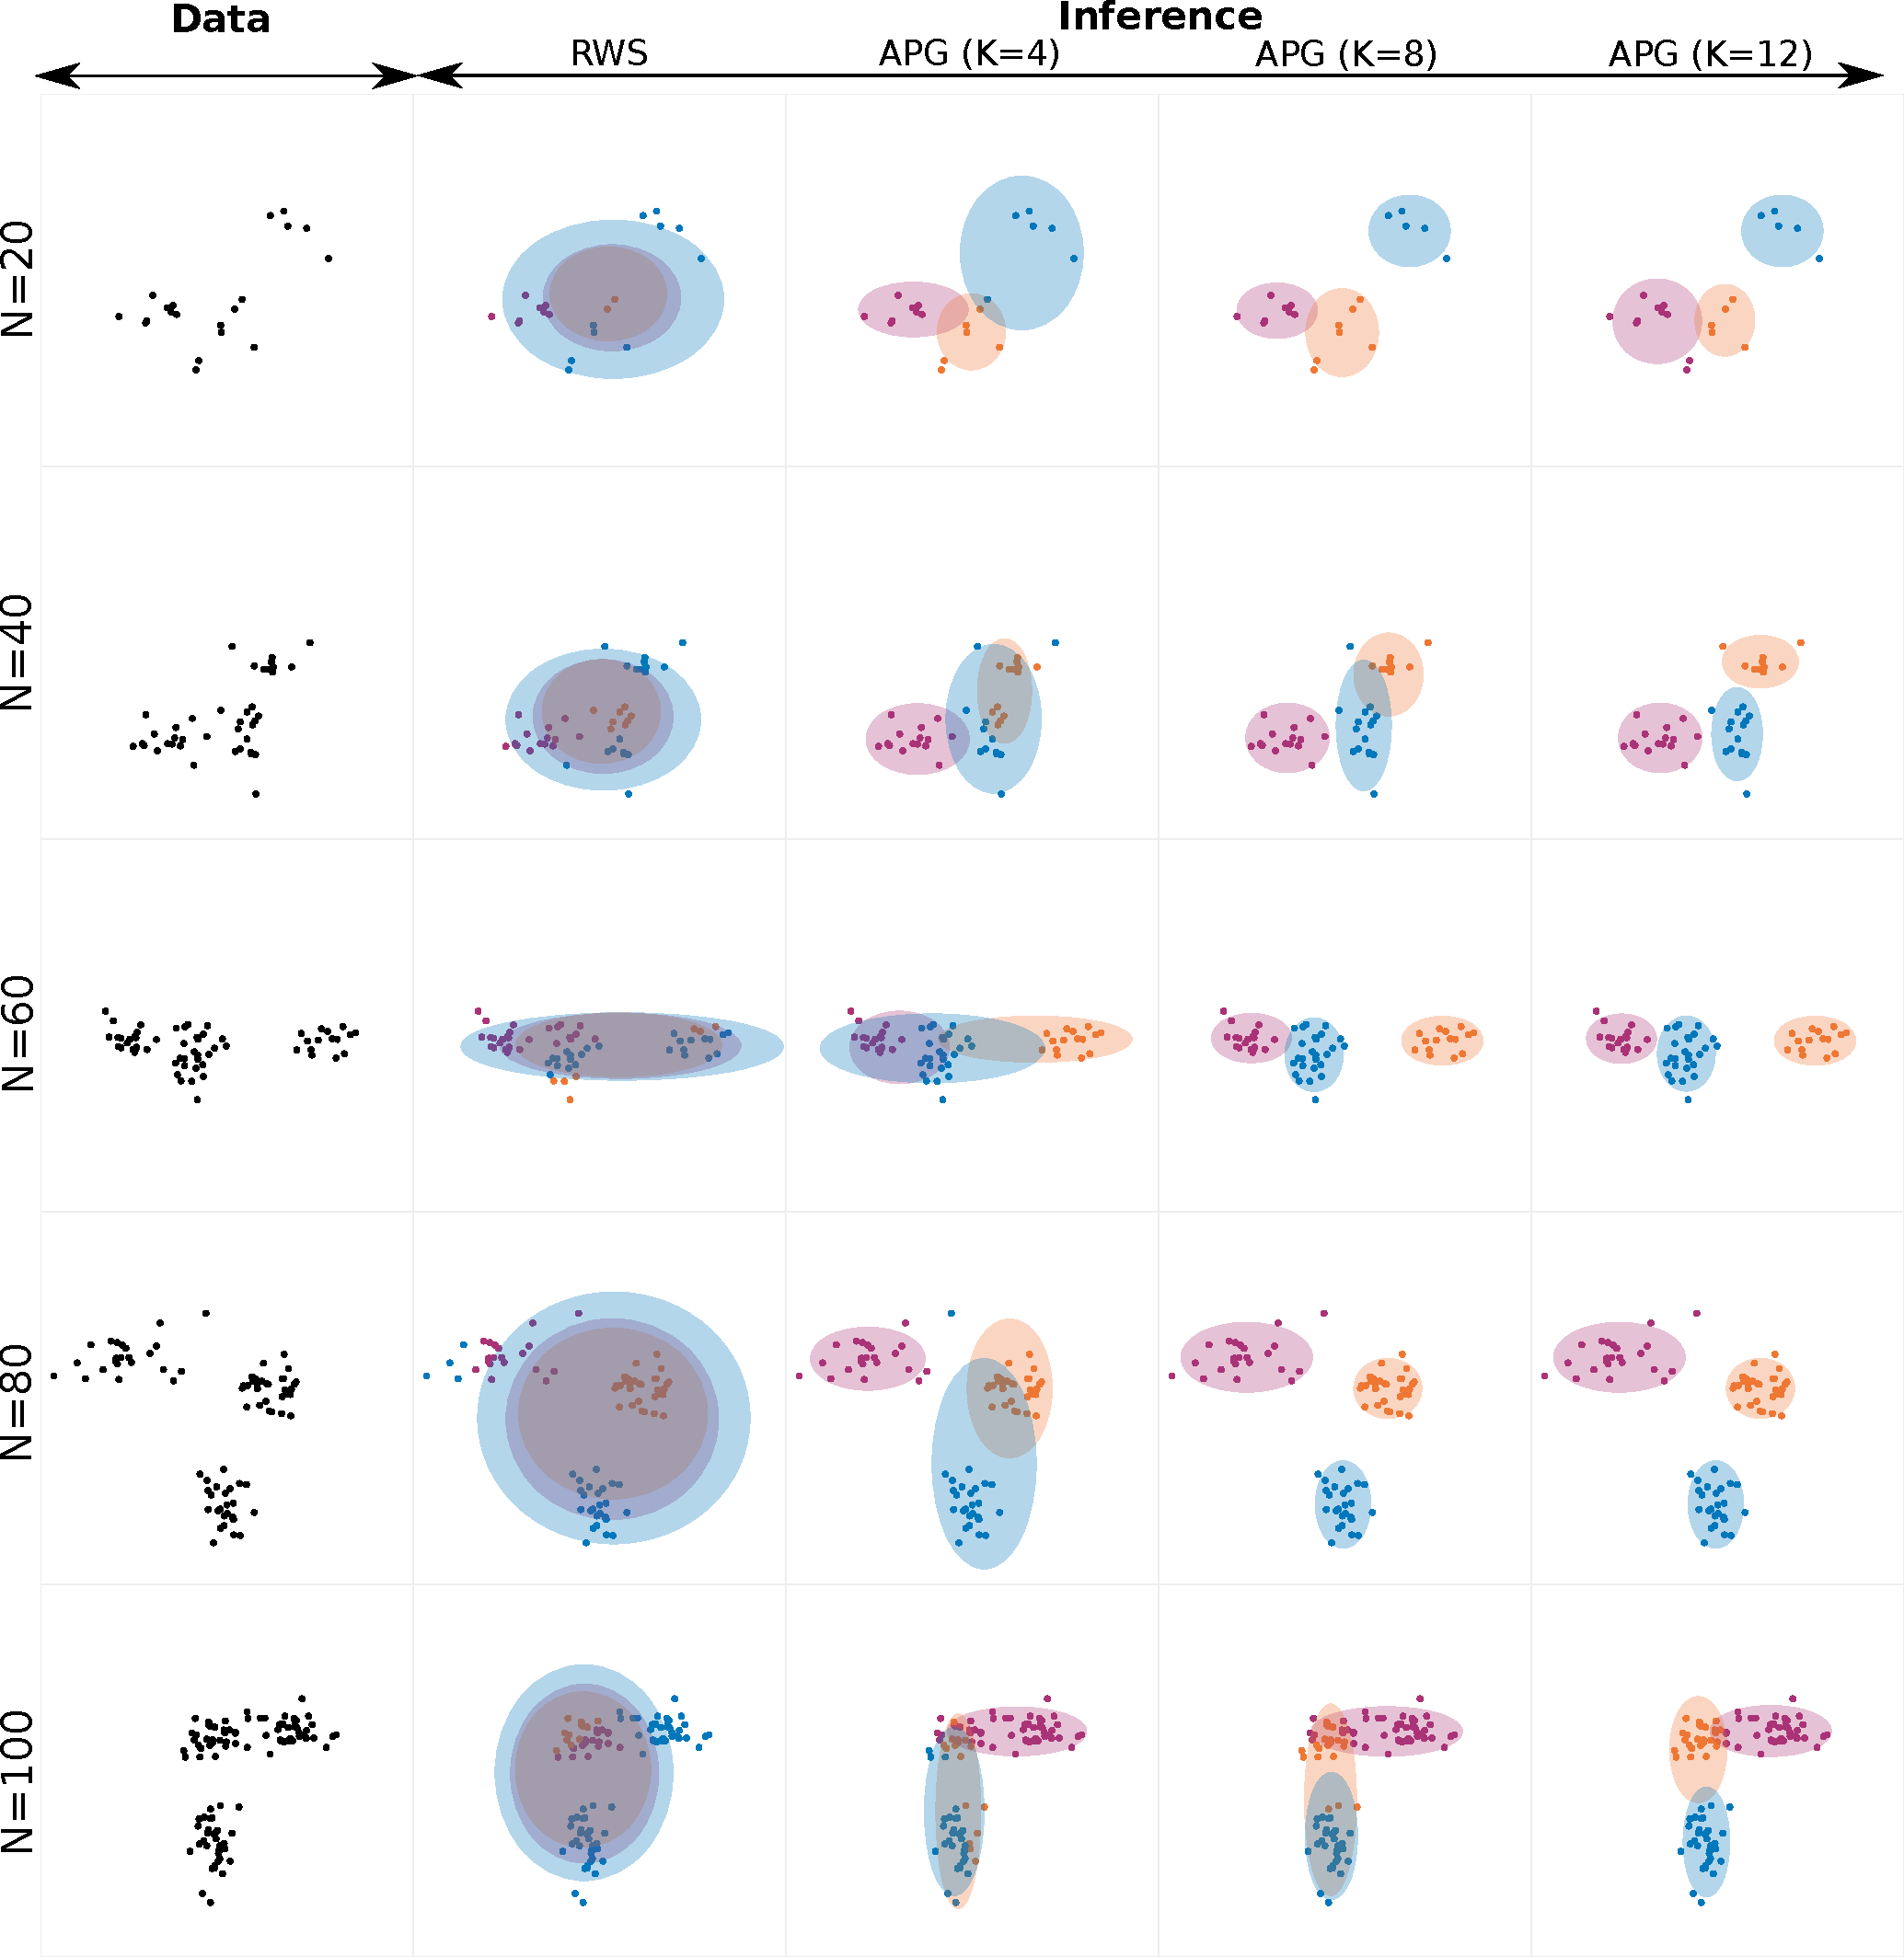
\includegraphics[width=67mm]{figures/gmm_samples.pdf}
  \vspace*{-1mm}
  \caption{GMM}
%   \label{samples-gmm}
  \vspace{-1ex}
  \end{subfigure}%
  \begin{subfigure}[t]{0.5\textwidth}
  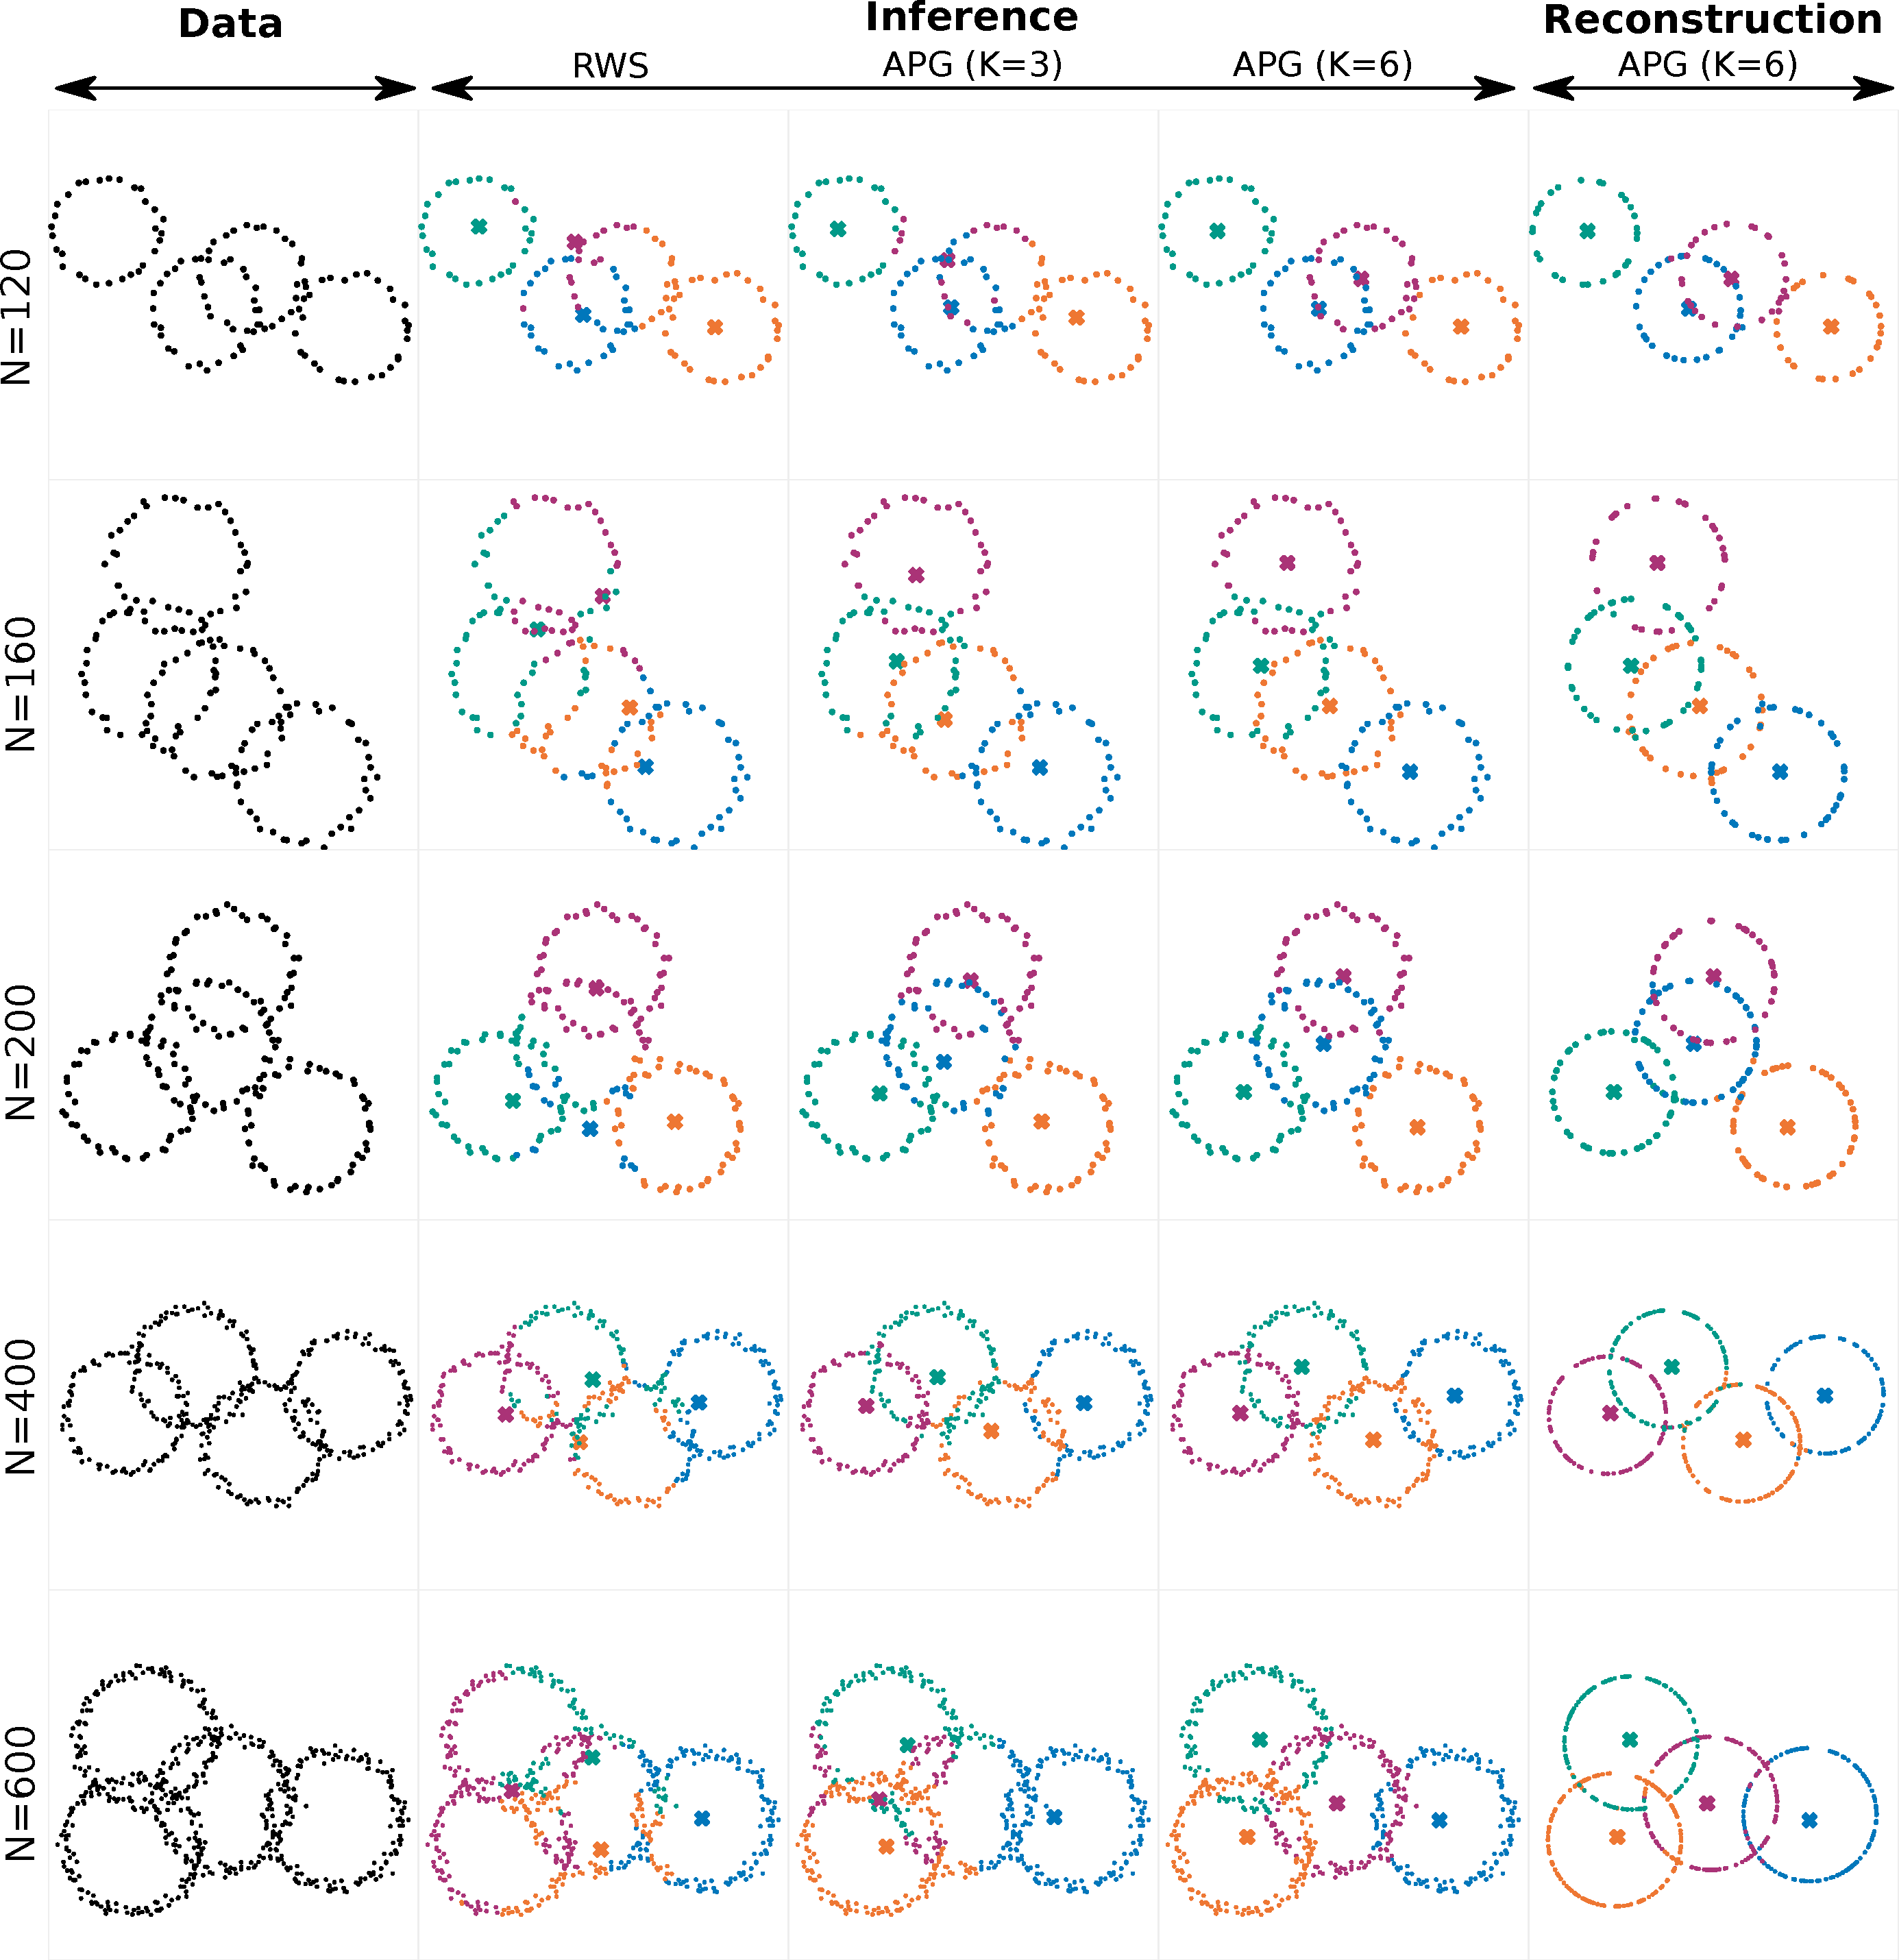
\includegraphics[width=67mm]{figures/dgmm_samples.pdf}
  \vspace*{-1mm}
  \caption{DGMM}
%   \label{samples-dgmm}
  \vspace{-1ex}
  \end{subfigure}
  \caption{Samples from the GMM and the DGMM. (\textbf{a}) GMM, the left column shows 5 test datasets with different number of data points. The subsequent columns show inference results by RWS, followed by results after 4, 8 and 12 APG updates. (\textbf{b}) DGMM, the left column shows 5 test datasets with different number of data points. The subsequent columns show the inference results by RWS, followed by results after 3 and 6 APG updates. The right column shows reconstructions from the learned generative model.}
  \label{samples-mixture}
\end{figure*}
\newpage
\subsection{Qualitative Results in Bouncing MNIST}
\label{appendix:samples-mnnist}
\begin{figure*}[!h]
  \centering
  \begin{subfigure}[t]{1.0\textwidth}
  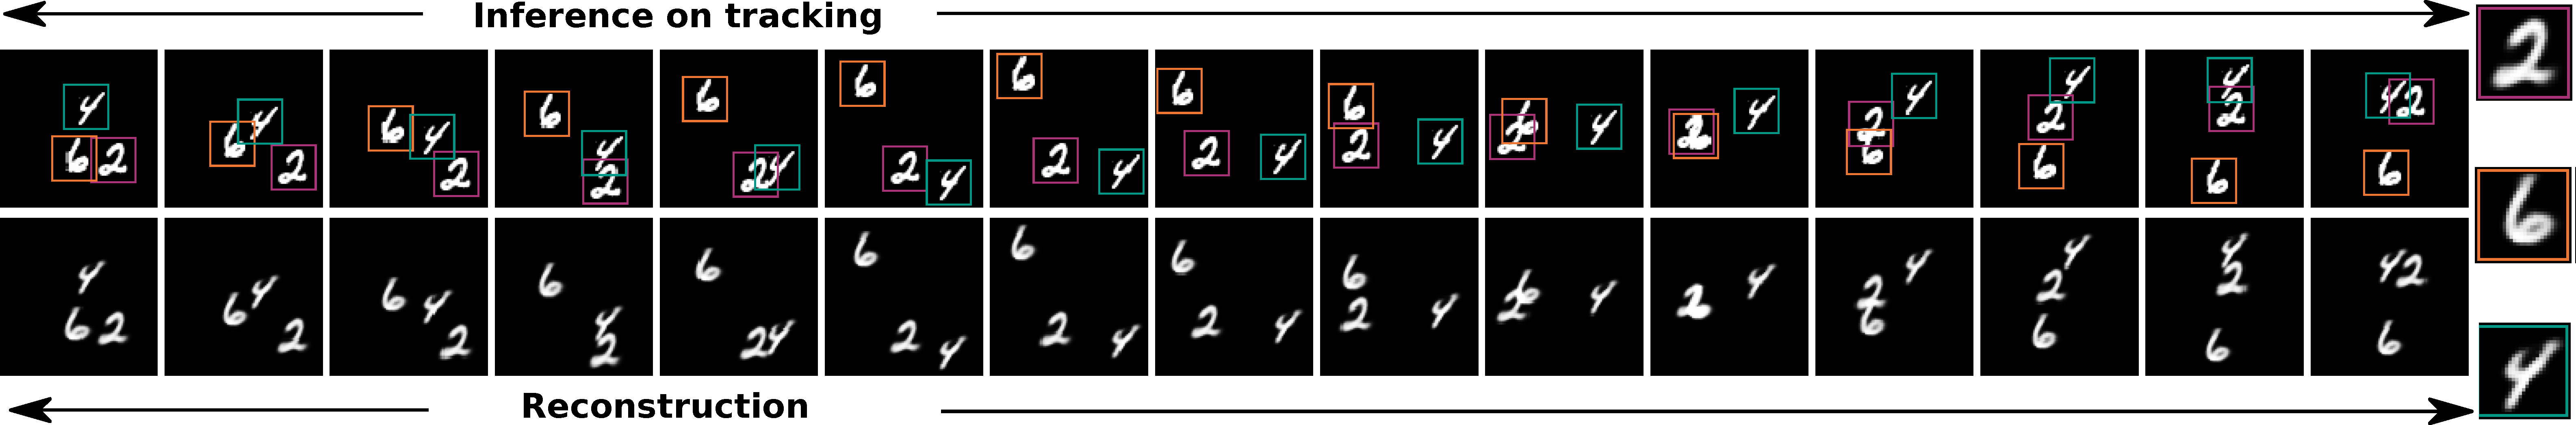
\includegraphics[width=1.0\textwidth]{figures/bmnist-3digits-samples.pdf}
%   \vspace*{-5mm}
%   \caption{3 digits.}
  \end{subfigure}
  %%%%%%%%%%%
  \begin{subfigure}[t]{1.0\textwidth}
  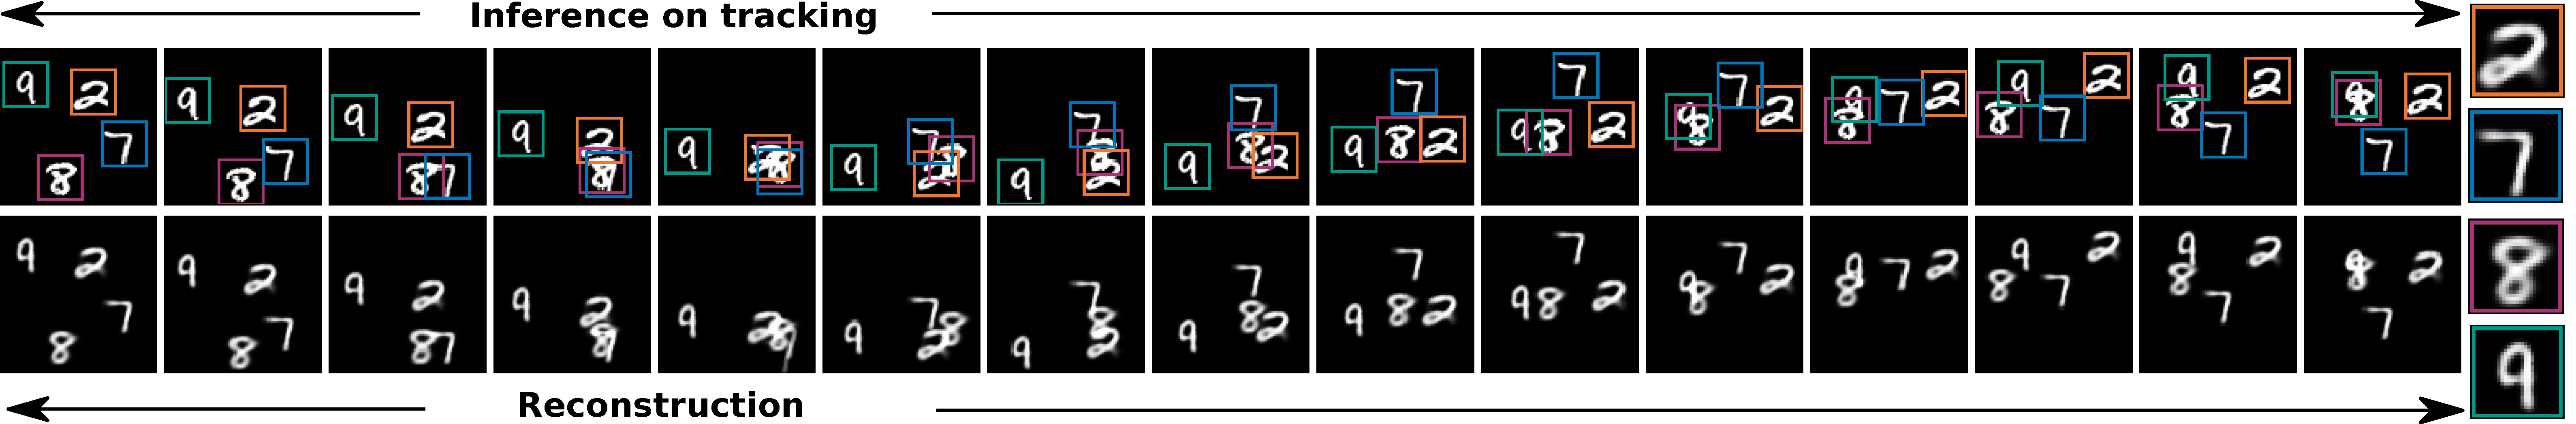
\includegraphics[width=1.0\textwidth]{figures/bmnist-4digits-samples.pdf}
%   \vspace*{-5mm}
%   \caption{4 digits.}
  \end{subfigure}
  %%%%%%%%%%%
  \begin{subfigure}[t]{1.0\textwidth}
  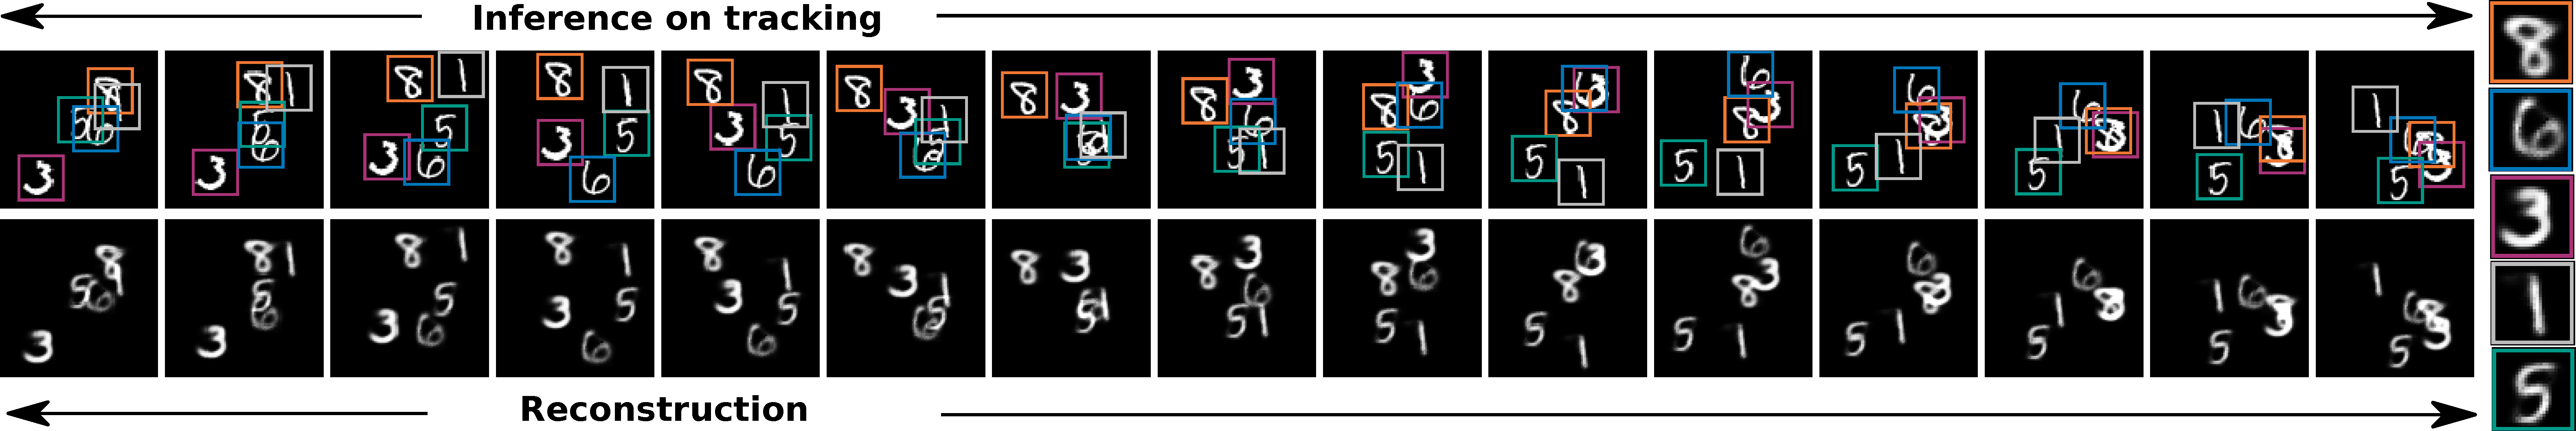
\includegraphics[width=1.0\textwidth]{figures/bmnist-5digits-samples.pdf}
%   \vspace*{-5mm}
%   \caption{5 digits.}
  \end{subfigure}
  \caption{Inferred digit trajectories and reconstructions for $D = 3$, $D = 4$, $D = 5$ digits for $T = 15$ for a model trained on $D = 3$ and $T = 10$.}
%   \label{mnist-qualitative}
\end{figure*}

The following are full reconstructions on test sets where time steps $T=100$ and number of digits $D=3, 4, 5$, respectively. In each figure, the 1st, 3rd, 5th, 7th, 9th rows show the inference results, while the other rows show the reconstruction of the series above.
\begin{figure*}[h!]
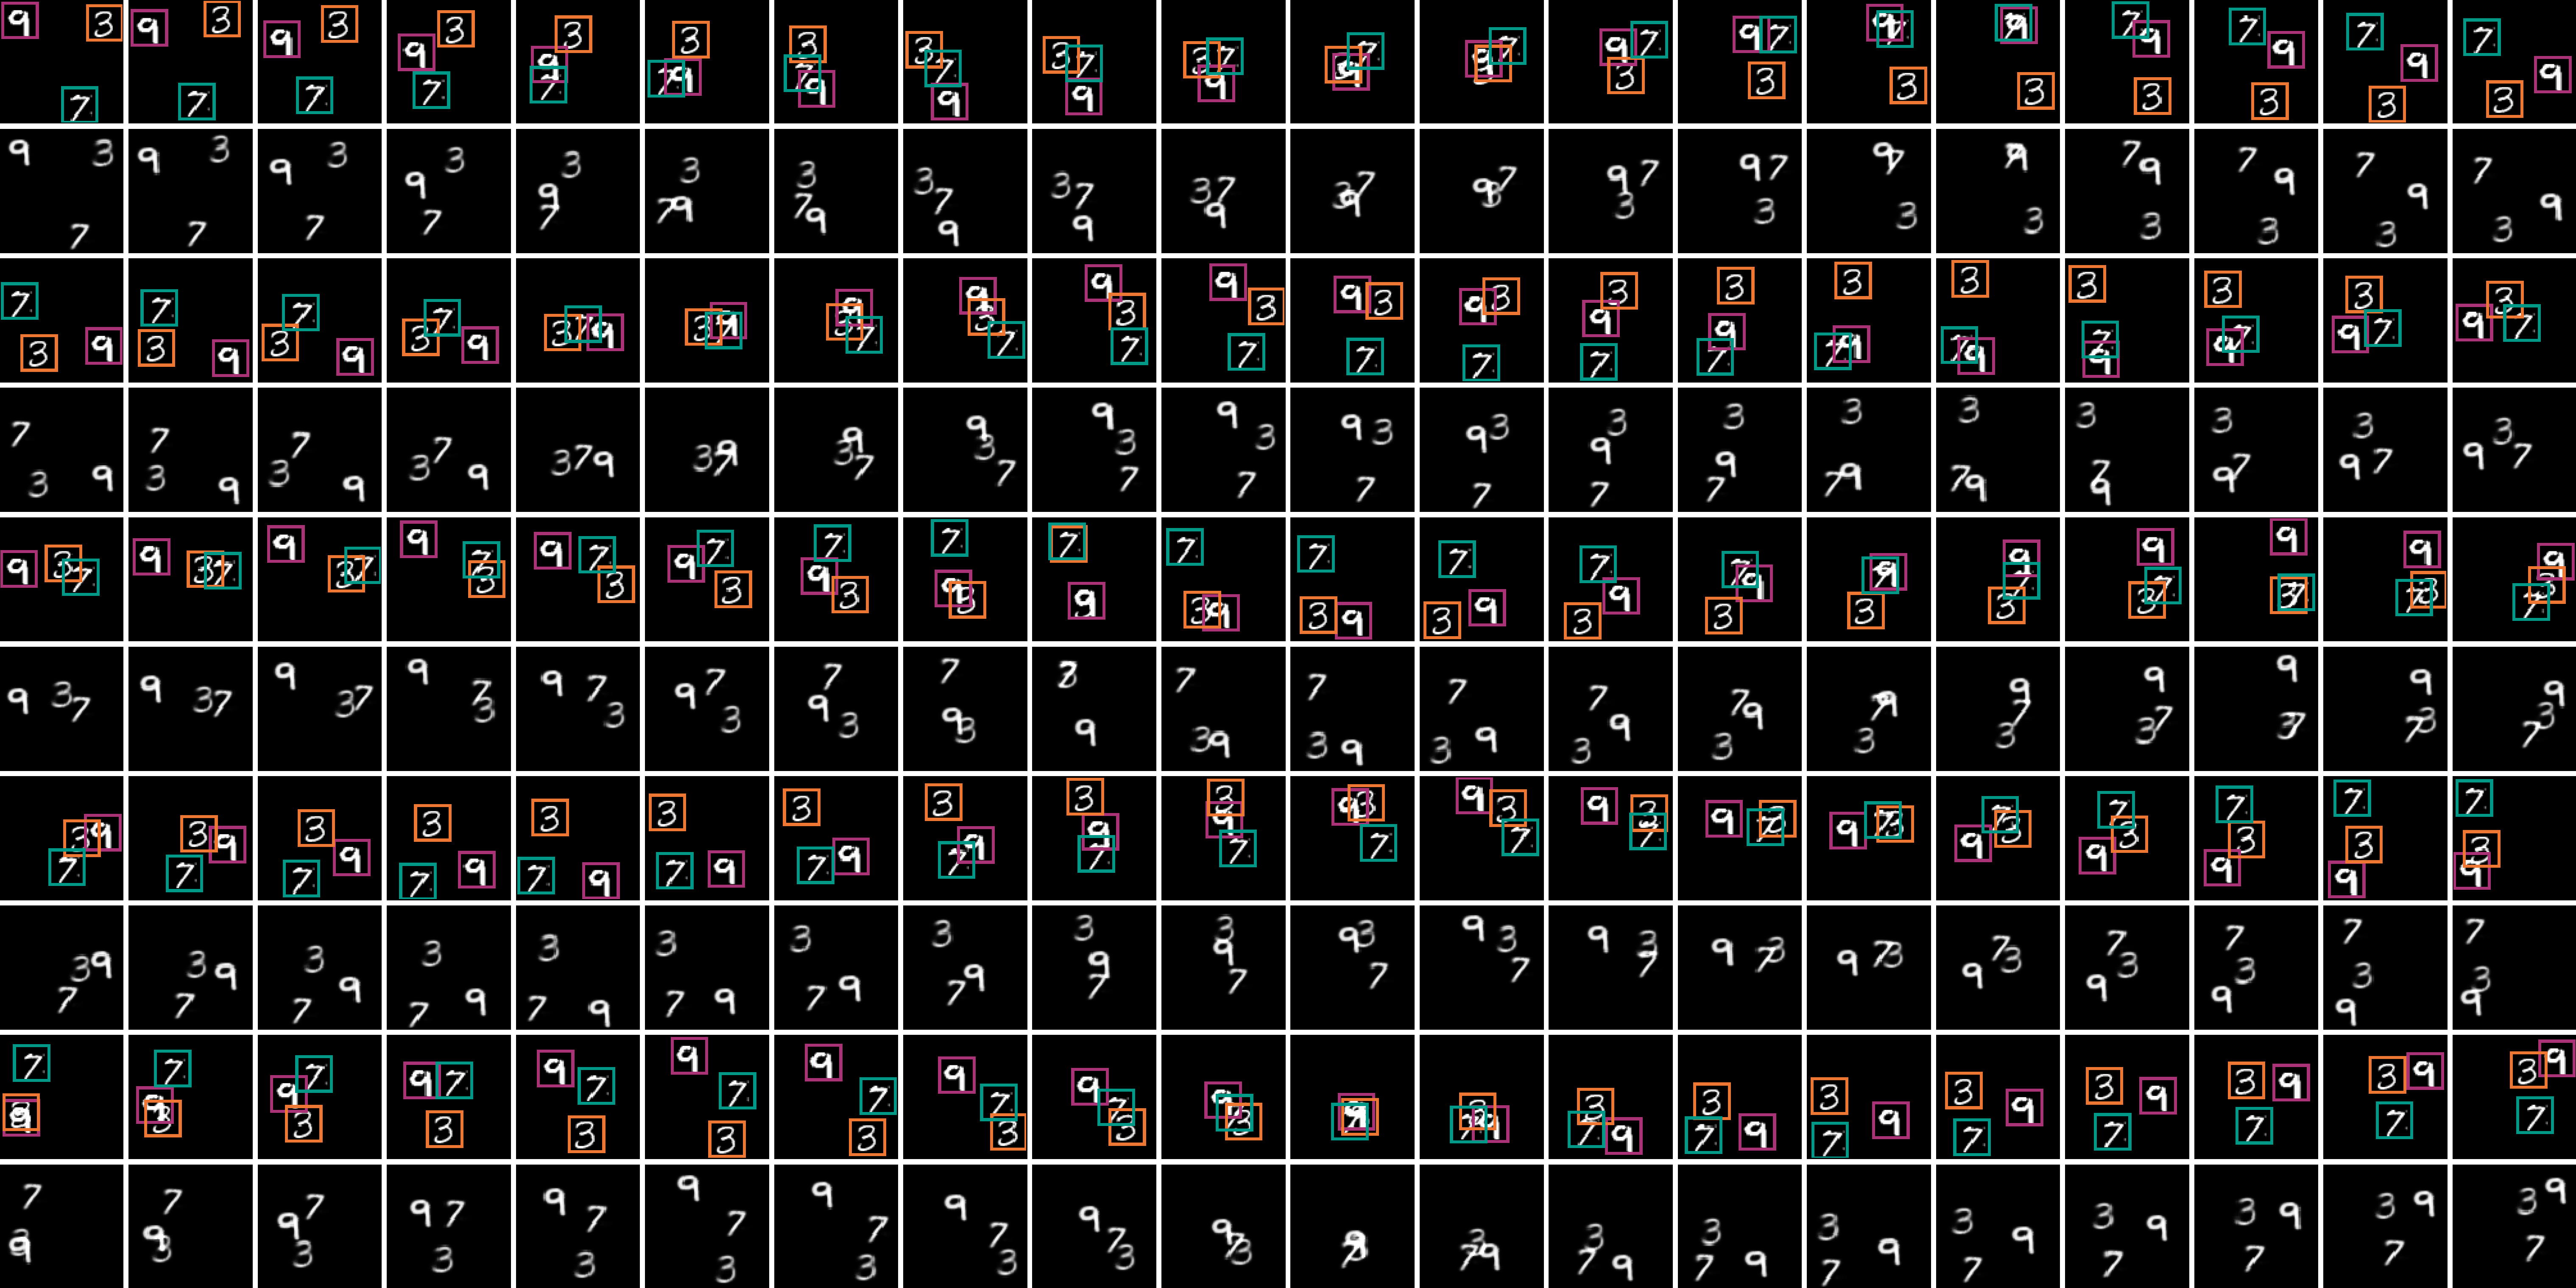
\includegraphics[width=\linewidth]{figures/T=100-D=3.pdf}
\caption{Full reconstruction for a video where $T=100, D=3$.}
\end{figure*}
\newpage
\begin{figure*}[h!]
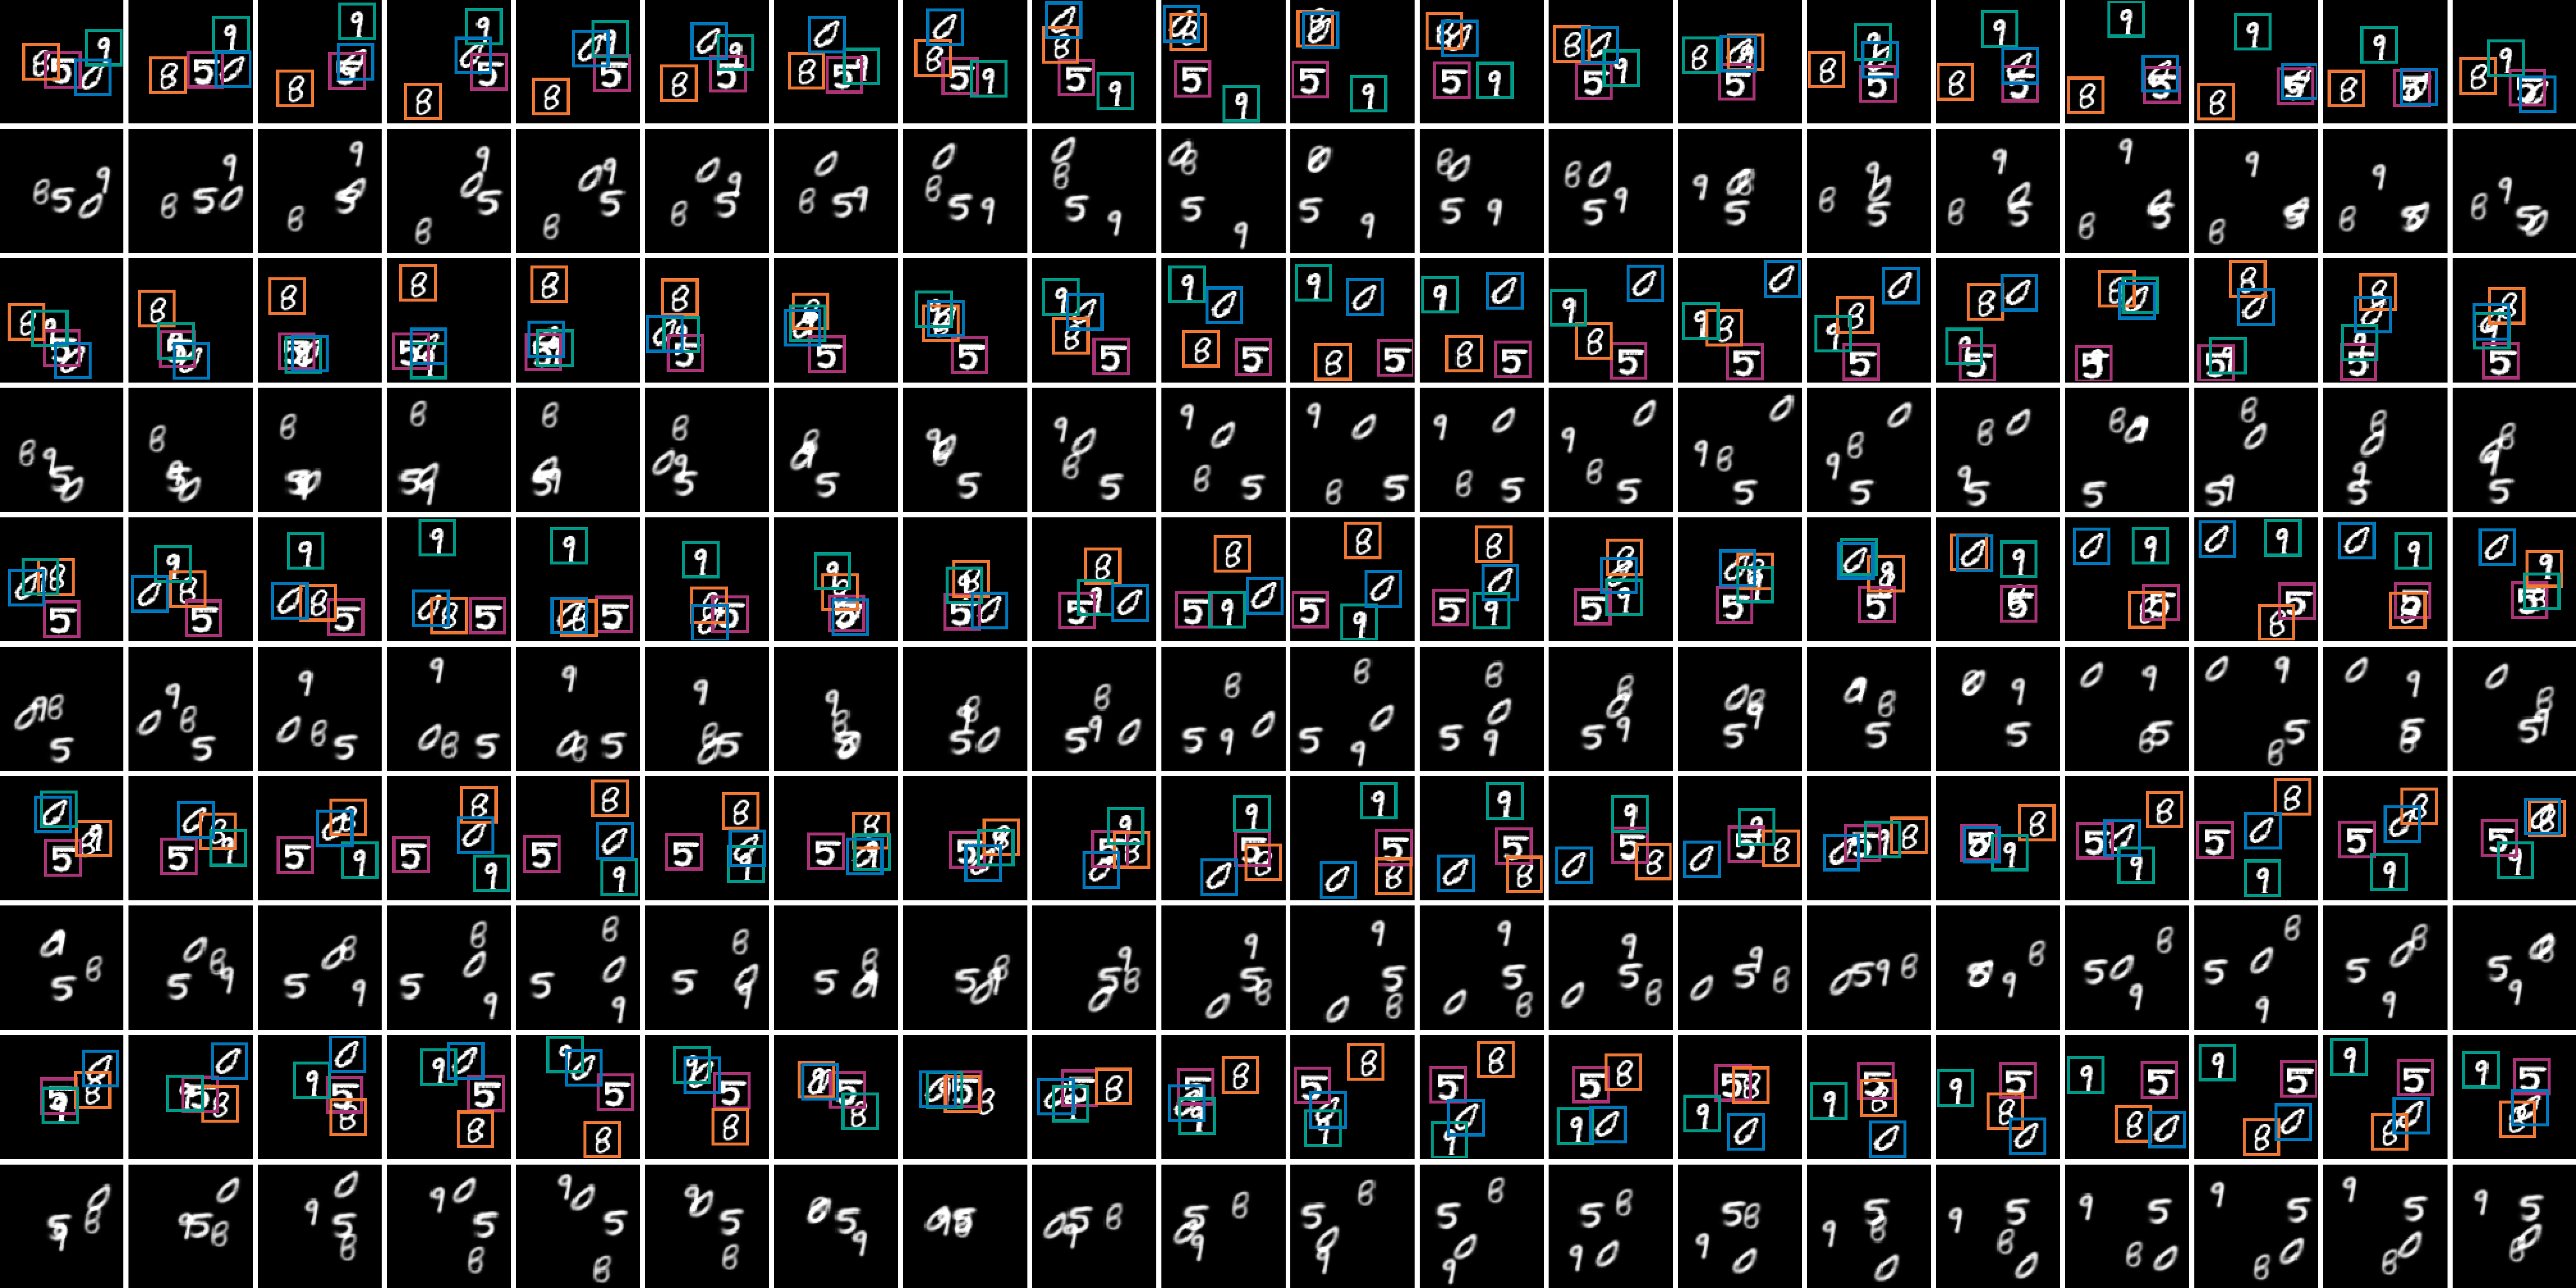
\includegraphics[width=\linewidth]{figures/T=100-D=4.pdf}
\caption{Full reconstruction for a video where $T=100, D=4$.}
\end{figure*}

\begin{figure*}[h!]
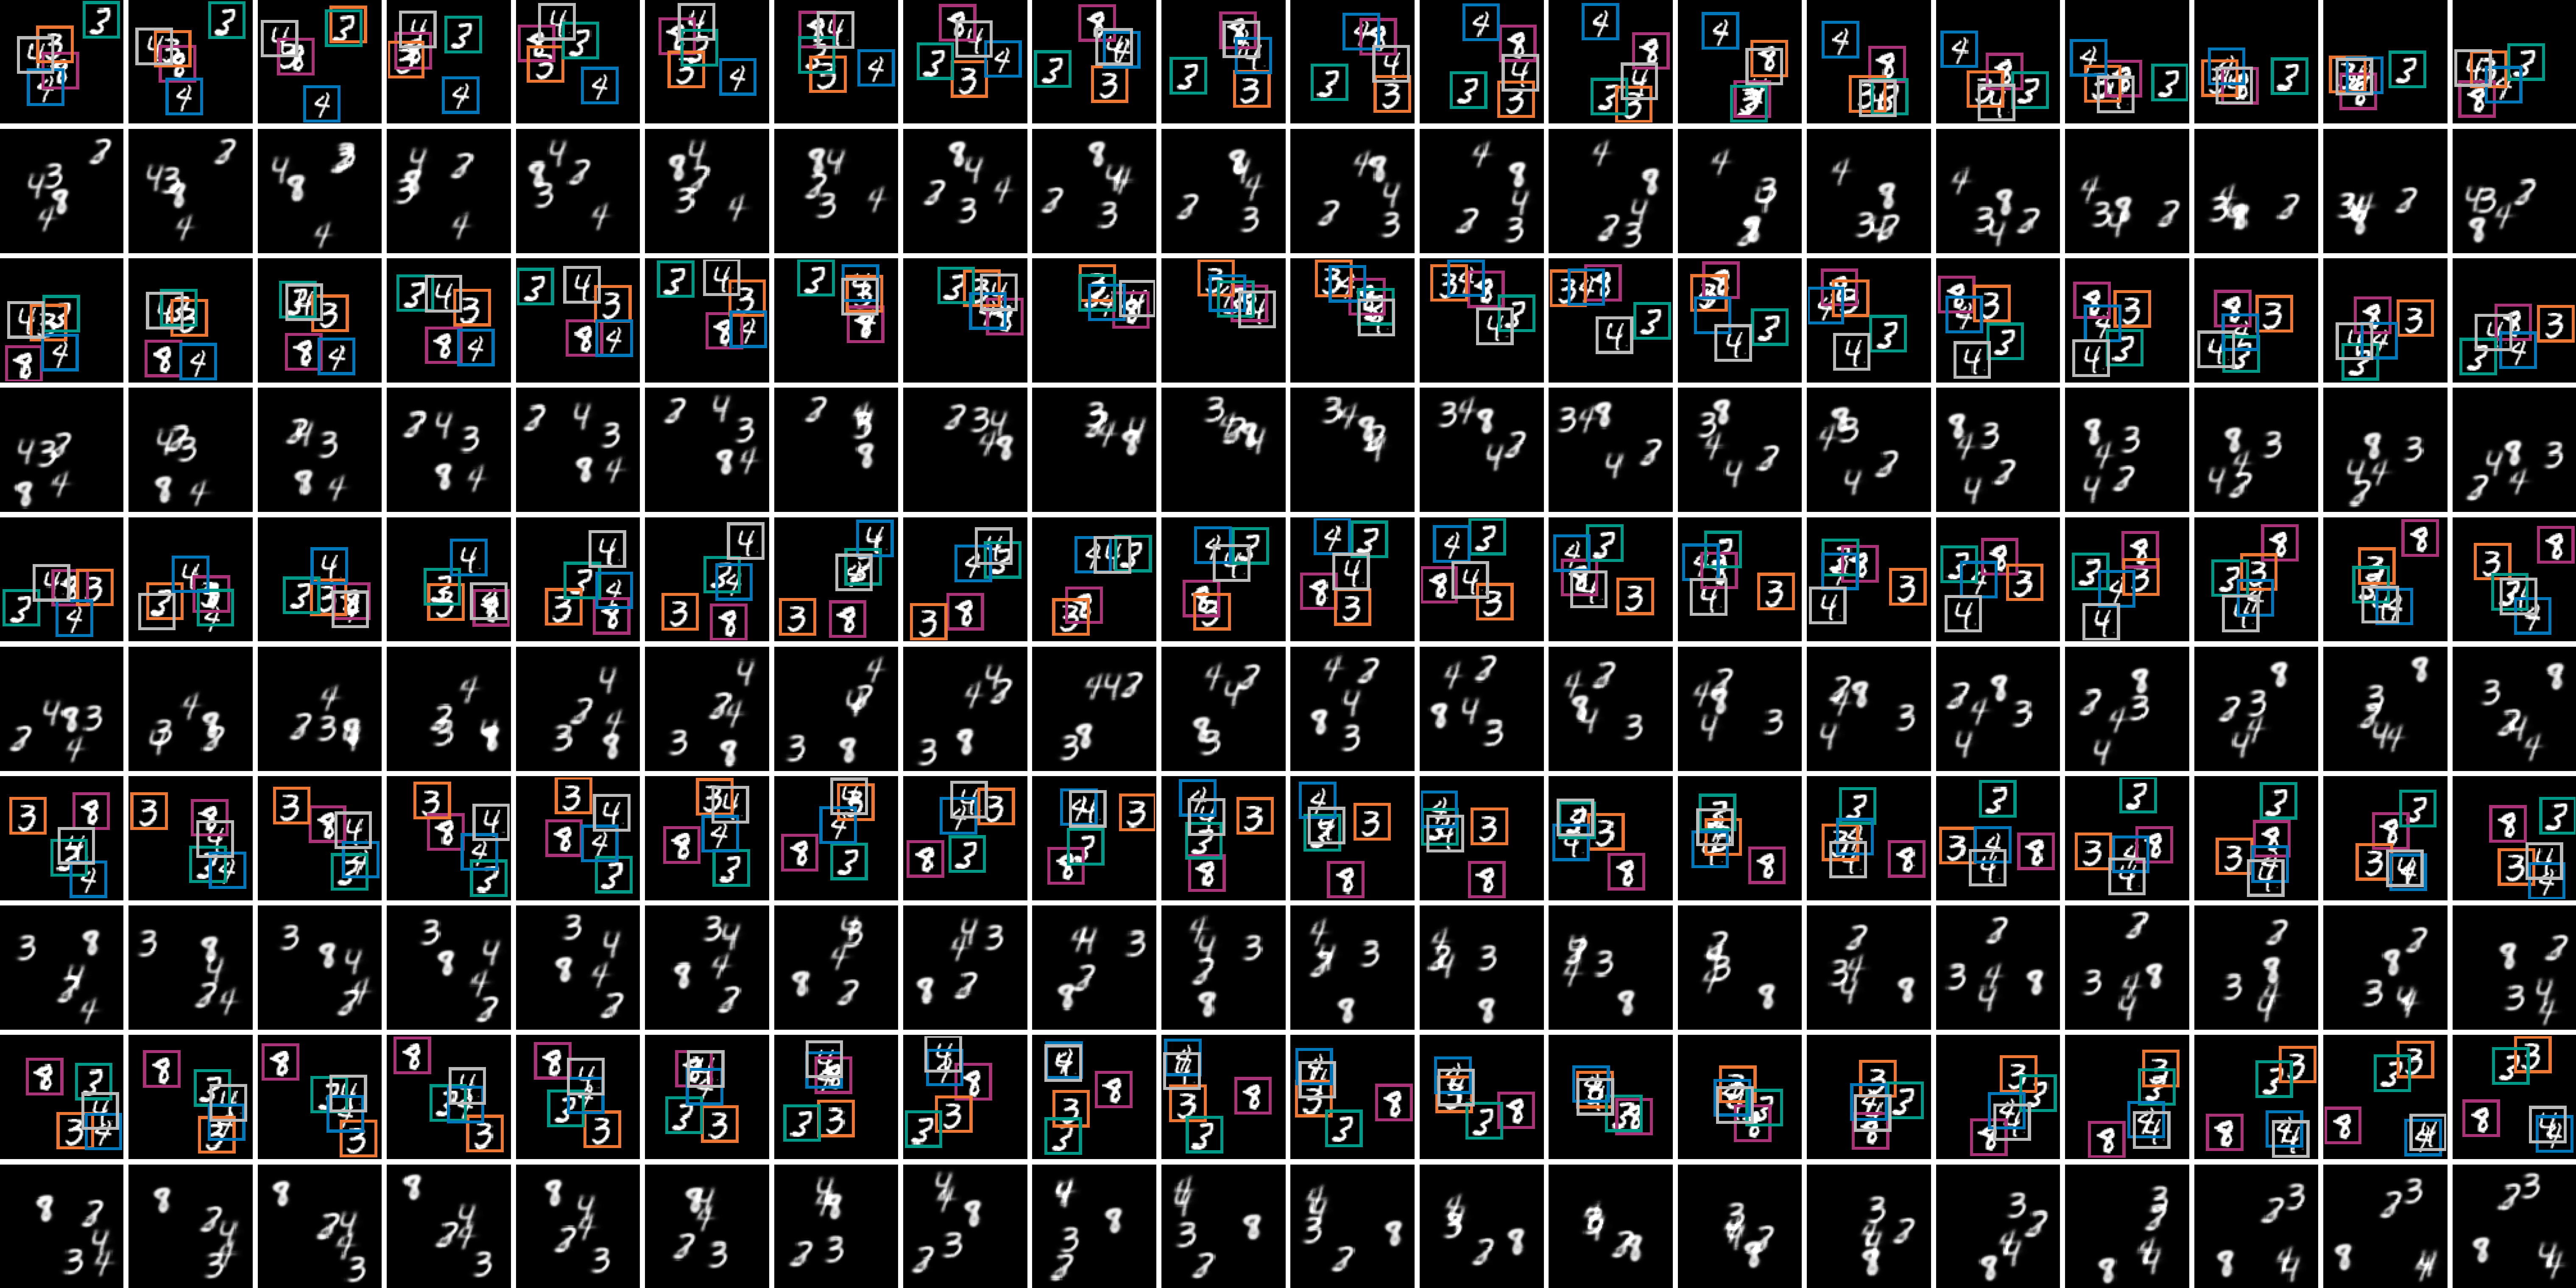
\includegraphics[width=\linewidth]{figures/T=100-D=5.pdf}
\caption{Full reconstruction for a video where $T=100, D=5$.}
\end{figure*}

% \begin{figure*}[h!]
% 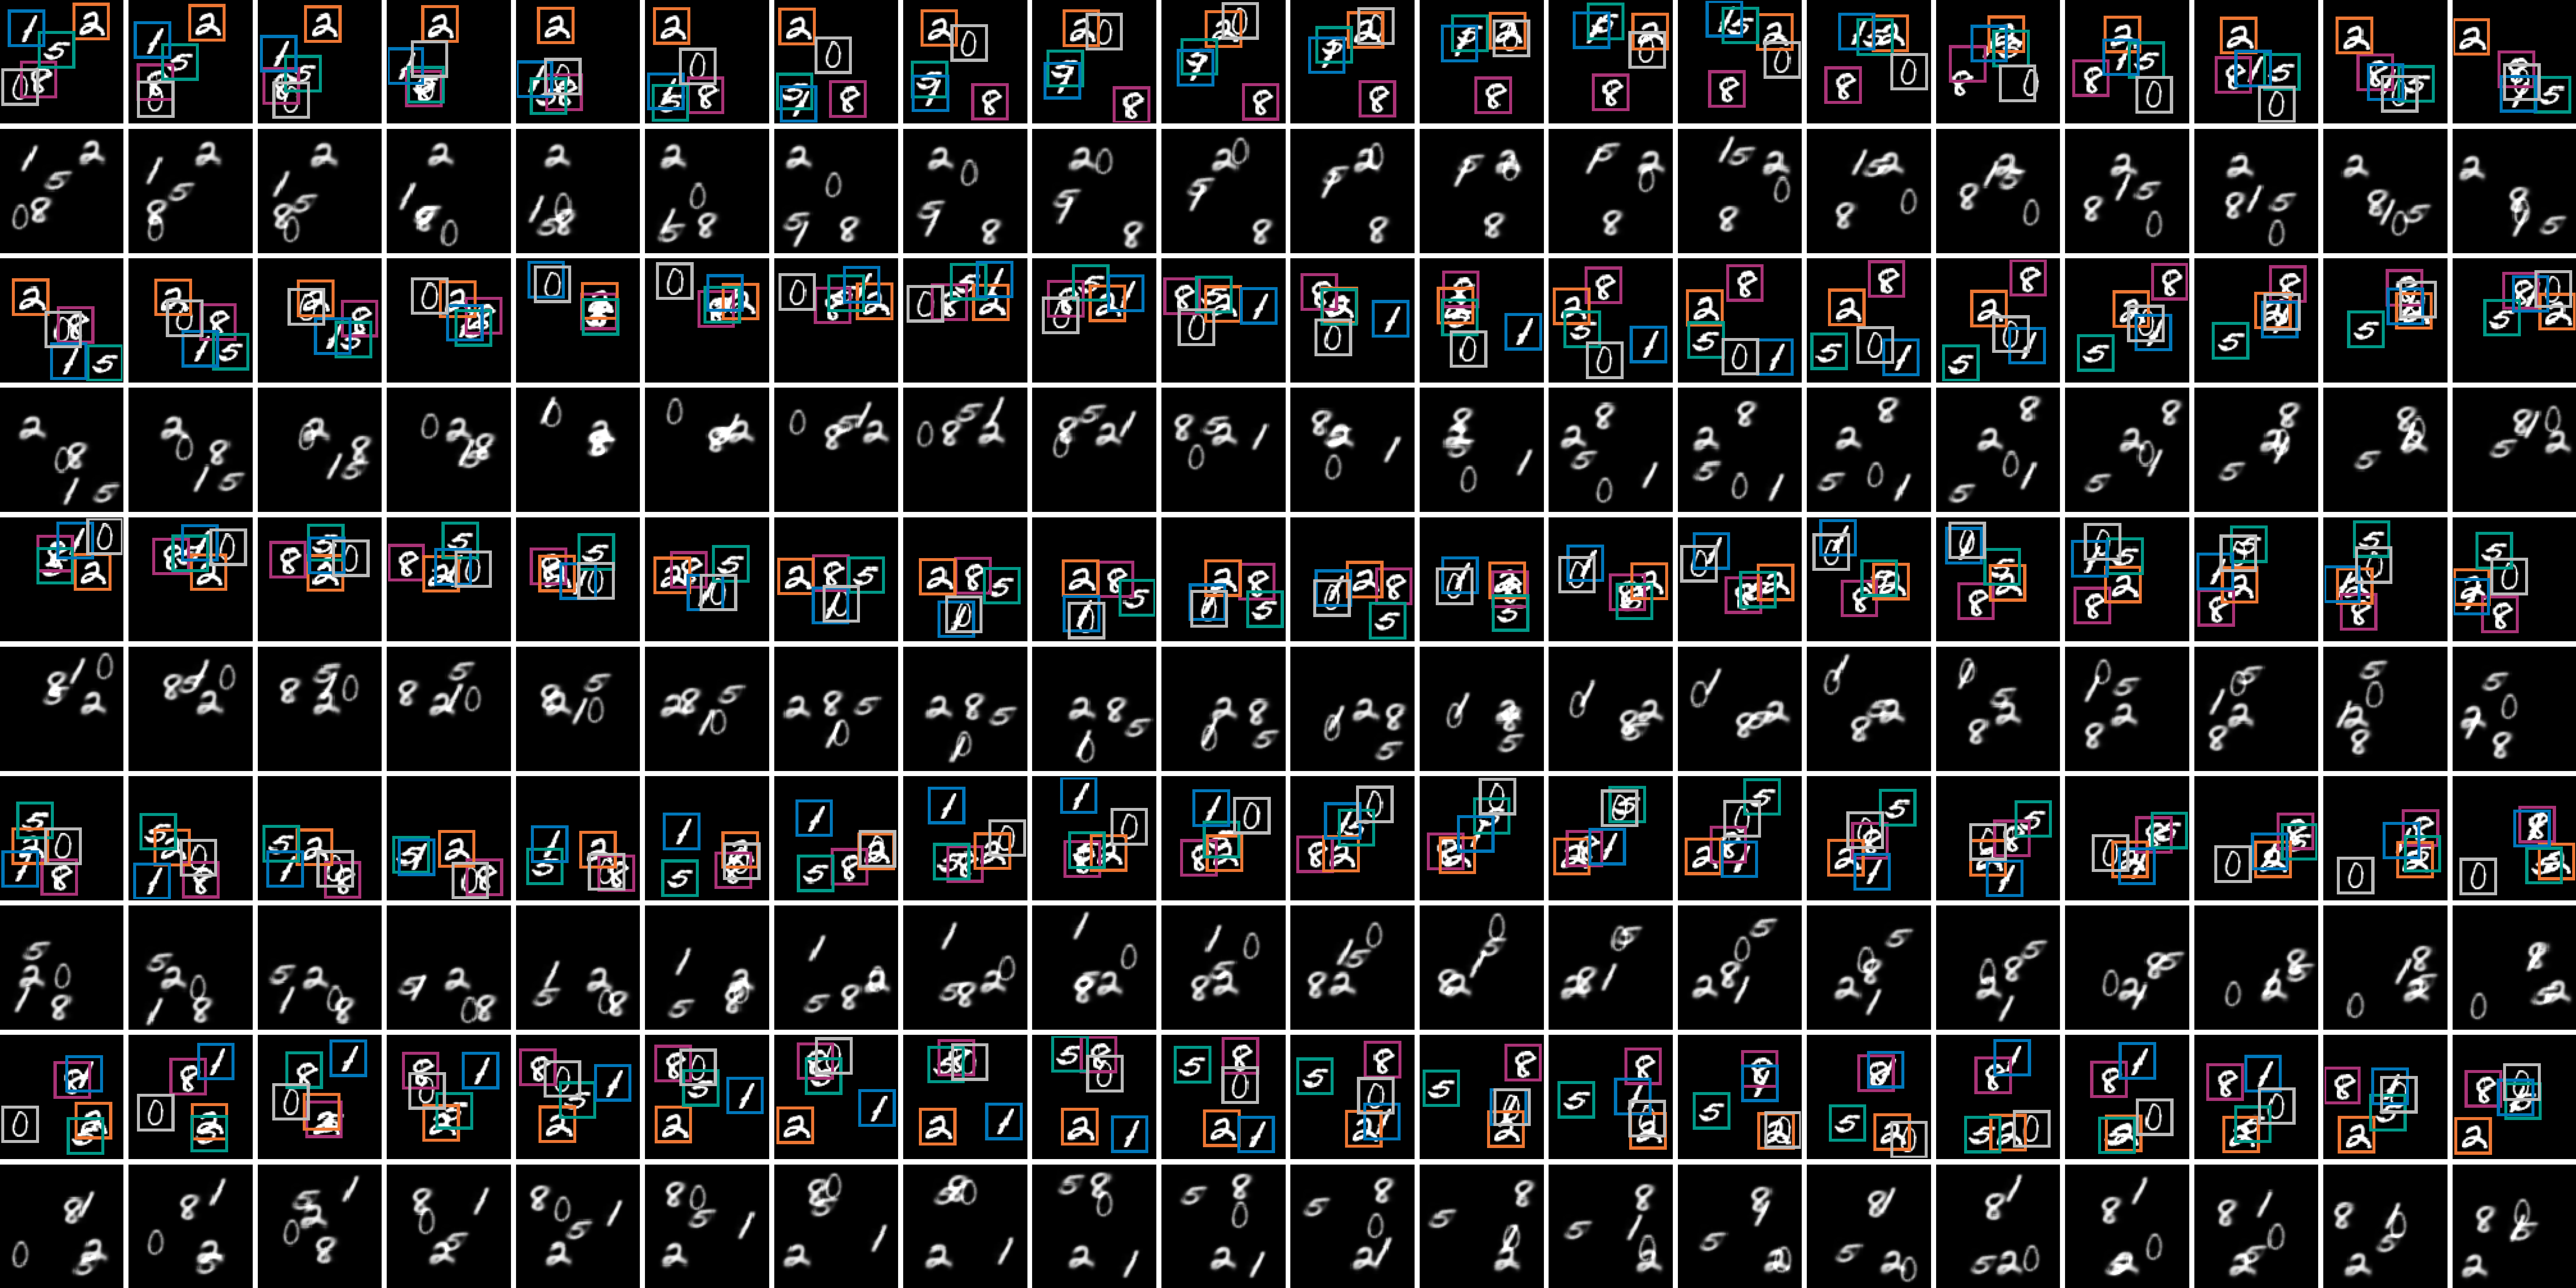
\includegraphics[width=\linewidth]{figures/T=100-D=5-2.pdf}
% \caption{Full reconstruction for a video where $T=100, D=5$.}
% \end{figure*}

\newpage
\subsection{Architecture of the Amortized Population Gibbs samplers}
\label{appendix:architecture}
\subsubsection{GMM}
\
\begin{table}[h]
    \centering
    \begin{tabular}{c|c|c}
    \toprule
     Layer 
     & 
    \multicolumn{2}{c}{$q_\f(\mu, \tau | x)$}
    \\
    \midrule
    Input
    & 
    \multicolumn{2}{c}{$\mathrm{Concat}[x_n\in\mathbb{R}^2]$}
    \\
    \hline
    1
    & \parbox{3cm}{\centering FC 2}
    & \parbox{3cm}{\centering FC 3 Softmax}
    \\
    \bottomrule
    \end{tabular}
    \label{arch-gmm-rws}
\end{table}

\begin{table}[h]
    \centering
    \begin{tabular}{c|c|c}
    \toprule
     Layer 
     & 
    \multicolumn{2}{c}{$q_\f(\mu, \tau | x, c)$}
    \\
    \midrule
    Input
    & 
    \multicolumn{2}{c}{$\mathrm{Concat}[x_n\in\mathbb{R}^2, c_n\in\mathbb{R}^3]$}
    \\
    \hline
    1
    & \parbox{3cm}{\centering FC 2}
    & \parbox{3cm}{\centering FC 3 Softmax}
    \\
    \bottomrule
    \end{tabular}
    \label{arch-gmm-global}
\end{table}

\begin{table}[h]
    \centering
    \begin{tabular}{c|c}
    \toprule
        Layer
        &
        $q_\f(c | x, \mu, \tau)$
        \\
    \midrule
    Input
    & 
    $\mathrm{Concat}[x_n\in\mathbb{R}^2, \mu_i\in\mathbb{R}^2]$\\
    \hline
    1
    & \parbox{4cm}{\centering FC 32 Tanh}\\
    \hline
    2 
    & FC 1, Intermediate Variable $o_i\in\mathbb{R}$ \\
    \hline
    3
    & $\mathrm{Concat}[o_i\in\mathbb{R}]$, Softmax ($c_n$) \\
    \bottomrule
    \end{tabular}
    \label{arch-gmm-local}
\end{table}

% \newpage
\subsubsection{DGMM}
\begin{table}[h]
    \centering
    \begin{tabular}{c|c|c}
    \toprule
        \textbf{Layer} &\multicolumn{2}{c}{$q_\f(\mu | x)$} \\
    \midrule
    Input &\multicolumn{2}{c}{$x_n\in\mathbb{R}^2$} \\
    \hline
    1 
    & 
     \parbox{4cm}{\centering FC 32 Tanh}
    & 
    \parbox{4cm}{\centering FC 32 Tanh}\\
    \hline
    2 
    &
    \parbox{4cm}{\centering FC 16 Tanh, $v_n\in\mathbb{R}$}
    & 
    \parbox{4cm}{\centering FC 4 Softmax, $\gamma_n\in\mathbb{R}^{3}$}\\
    \hline
    3 &\multicolumn{2}{c}{$T_n := \gamma_n \tens{} v_n\in\mathbb{R}^{3\times16}$} \\
    \hline
    4 &\multicolumn{2}{c}{$\mathrm{Concat}[\sum_n^N T_n[i], \mu_0\in\mathbb{R}^2, \mathrm{Diag}(\sigma_0^2 I)\in\mathbb{R}^2], i=1,2,3,4$} \\
    \hline
    5 &\multicolumn{2}{c}{FC 2$\times$32 Tanh} \\
    \hline
    6 &\multicolumn{2}{c}{FC 2$\times$8 ($\mu_{1:I}$)} \\
    \bottomrule
    \end{tabular}
    \label{arch-dgmm-rws}
\end{table}

\begin{table}[h]
    \centering
    \begin{tabular}{c|c|c}
    \toprule
        \textbf{Layer} &\multicolumn{2}{c}{$q_\f(\mu | z, c)$} \\
    \midrule
    Input &\multicolumn{2}{c}{$\mathrm{Concat}[x_n\in\mathbb{R}^2, c_n\in\mathbb{R}^3]$} \\
    \hline 
    1 
    & 
    \parbox{4cm}{\centering FC 32 Tanh}
    & 
    \parbox{4cm}{\centering FC 32 Tanh} \\
    \hline 
    2 
    &
    \parbox{4cm}{\centering FC 16, $v_n\in\mathbb{R}$}
    & 
    \parbox{4cm}{\centering FC 4 Softmax, $\gamma_n\in\mathbb{R}^{3}$}
    \\
    \hline
    3 & \multicolumn{2}{c}{$T_n := \gamma_n \tens{} v_n\in\mathbb{R}^{3\times16}$}  \\
    \hline
    4 & \multicolumn{2}{c}{$\mathrm{Concat}[\sum_n^N T_n[i], \mu_0\in\mathbb{R}^2, \mathrm{Diag}(\sigma_0^2 I)\in\mathbb{R}^2], i=1,2,3,4$} \\
    \hline 
    5 &\multicolumn{2}{c|}{FC 2$\times$32 Tanh} \\
    \hline
    6 &\multicolumn{2}{c|}{FC 2$\times$2 ($\mu_i$)} \\
    \bottomrule
    \end{tabular}
    \label{arch-dgmm-global}
\end{table}


\begin{table}[h]
    \centering
    \begin{tabular}{c|c}
    \toprule
        \textbf{Layer} &
        $q_\f(c | z, \mu)$ \\
    \midrule
    Input  
    & 
    $\mathrm{Concat}[x_n\in\mathbb{R}^2, \mu_i\in\mathbb{R}^2]$\\
    \hline 
    1  
    & 
    FC 32 Tanh\\
    \hline 
    2
    & 
    \parbox{4cm}{FC 1, Intermediate Variable $o_i\in\mathbb{R}$} \\
    \hline
    3 & 
    \parbox{4cm}{$\mathrm{Concat}[o_i\in\mathbb{R}]$, Softmax ($c_n$)} \\
    \bottomrule
    \end{tabular}
    \label{arch-dgmm-assignment}
\end{table}

\begin{table}[h]
    \centering
    \begin{tabular}{c|c}
    \toprule
        \textbf{Layer} &
        $q_\f(\alpha | x, z, \mu)$ \\
    \midrule
    Input  
    & 
    $x_n - \mu_i \in\mathbb{R}^2 | z_n = i$\\
    \hline 
    1  
    & 
    FC 32 Tanh\\
    \hline 
    2
    & 
    \parbox{4cm}{FC 1 Tanh} \\
    \bottomrule
    \end{tabular}
    \label{arch-dgmm-angle}
\end{table} 

\begin{table}[h]
    \centering
    \begin{tabular}{c|c}
    \toprule
    \textbf{Layer}
    &
    $p_q(x | \mu, c, \alpha)$ \\
    \midrule
    Input
    &
    $\mathrm{Concat}[\alpha_n, c_n]\in\mathbb{R}^5$ 
    \\
    \hline
    1
    &
    FC 32 Tanh \\
    \hline
    2
    &
    FC 2 Tanh ($\mu_n$, fixed $\sigma_\epsilon$)\\
    \bottomrule
    \end{tabular}
    \label{arch-dgmm-decoder}
\end{table}
\newpage
\subsubsection{Bouncing MNIST}

\begin{table}[h]
\centering
\label{arch-bmnist-decoder}
\begin{tabular}{c|c}
    \toprule
    \textbf{Layer} & $p_\q(x | z^{\mathrm{what}}, z^{\mathrm{where}})$ \\
    \midrule
    Input & $z^{\mathrm{what}}_i \in\mathbb{R}^{10}$
    \\
    \hline
    1 &
    FC 200 ReLU \\
    \hline
    2 &
    FC 400 ReLU \\
    \hline
    3 & digit $d_i\in\mathbb{R}^{784}$\\
    \hline
    4 & ST($d_{i}, z^{\mathrm{where}}_{i, t}) \in\mathbb{R}^{9276}, i=1...,i, t=1...,T$ \\
    \bottomrule
\end{tabular}
\end{table}

\begin{table}[h]
\centering
\begin{tabular}{c|c}
    \toprule
    \textbf{Layer} & $q_\f(z^{\mathrm{what}} | z^{\mathrm{where}})$ \\
    \midrule
    Input & $x_t\in\mathbb{R}^{9276}, z^{\mathrm{where}}_{i, t}\in\mathbb{R}^{2}, i=1...,I, t=1...,T$
    \\
    \hline
    1 & 
    ST($x_t$, $z^{\mathrm{where}} _{i, t}$) $\in\mathbb{R}^{784}, i=1,..,I, t=1,...,T$  \\
    \hline
    2 &
    FC 400 ReLU \\
    \hline
    3 &
    FC 200 ReLU \\
    \hline
    4 & $z^{\mathrm{what}}_{i, t} \in\mathbb{R}^{10}, i=1,..,I, t=1,...,T$  \\
    \hline
    5 &
    Mean($z^{\mathrm{what}}_{1, t}$, $1:T$) $\in\mathbb{R}^{10}, i=1,...,I$\\
    \bottomrule
    \label{arch-bmnist-enc-what}
\end{tabular}
\end{table}

\begin{table}[h]
    \centering
    \begin{tabular}{c|c}
     \toprule
    \textbf{Layer} & $q_\f(z^{\mathrm{where}} | z^{\mathrm{what}})$ \\
    \midrule
    Input &
    $x_t\in\mathbb{R}^{9276}$, $z^{\mathrm{what}}_{i, t}, i=1,.., t=1,..,T$ \\
    \hline
    1 & 
    Conv2d($x_t$, $z^{\mathrm{what}}_{i, t}$)$\in\mathbb{R}^{4638}$, $i=1,.., t=1,..,T$ \\
    \hline
    2  &
    FC 400 Tanh \\
    \hline
    3 & $2\times$ FC 200 Tanh \\
    \hline
    4 &
    $2\times2$ Tanh 
    \\
    \bottomrule
    \end{tabular}
    \label{arch-bmnist-enc-where}
\end{table}
\end{document}
